\chapter{Background\label{chap2}}

\section{Real-time Systems}
A real-time embedded system consists of computational tasks that are bounded by time constraints. The time constraint is dictated by the environment in which the real-time system is integrated. 
Kopetz \cite{Kopetz:2011:RSD:1995310} has defined the real-time system as follows:

\emph{"real-time system is a computer system in which the correctness of the system behavior depends not only on the logical results of the computations but also on the physical instant at which these results are produced"}. 

The system works correctly as long as the results are logically correct and produced within prescribed timing constraints. 
A task is a piece of workload that the real-time system has to execute within prescribed timing constraints. 
The real-time computing system can be designed to perform a single or multiple tasks. 
The behavior of a real-time system can be well understood by understanding characteristics of real-time tasks. 
Every real-time task is imposed by a time constraint called \emph{deadline}. 
The real-time system is supposed to complete real-time tasks before the deadline of a task passes.
The time instance when a real-time task becomes ready for execution is called \emph{release time}. 
The difference between release time and the instant of time when the real-time task handler is scheduled to compute workload is called latency.
The maximum or worst-case time needed to complete the task after it is scheduled is called \emph{response time} also called worst-case execution time (WCET). 
Figure \ref{fig-rt-task-param} demonstrates response time of real-time task under normal circumstances assuming latency is zero. 

\begin{figure}[!htb]
\begin{center}
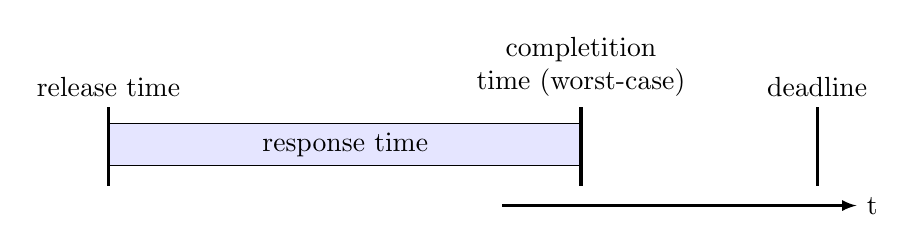
\begin{tikzpicture}

\node at (0,0.25)[rectangle, draw=black, fill=blue!10, minimum height = 0.5cm, minimum width = 6cm, anchor=south west] (resptime) {response time};
\draw[black, very thick, solid] (0,0) -- (0,1) node [above] {release time};
\draw[black, very thick, solid] (6,0) -- (6,1) node [above, text width=4cm, text centered] {completition time (worst-case)};
\draw[black, very thick, solid] (9,0) -- (9,1) node [above] {deadline};

%\node (rtlabel) at (5,-1.5) {response time};
\begin{scope}[>=latex]
	%%\draw [thick, ->] (rtlabel) to [bend left=45] (resptime.center);
	\draw[black, thick, ->] (5,-0.25) -- (9.5,-0.25) node [right] {t};
\end{scope}
\end{tikzpicture}
\end{center}
\ifreport
\caption{response time of real-time task}
\fi
\label{fig-rt-task-param}
\end{figure}


Deadline of a real-time task is categorized into three types: soft, firm and hard. 
The deadline is firm, if missing the deadline makes the result unusable, soft if the result is still usable. 
A hard deadline means missing it would disrupt the system functionality resulting in a failure of the system.
Real-time systems are often categorized into soft and hard real-time systems based on the type of deadlines tasks are supposed to meet.
A hard real-time system consists of at least one task with a hard deadline. 
A safety-critical system is a hard real-time system where system failure can cause a disaster.
On contrary, all tasks in soft real-time system have soft or firm deadlines. 
Nevertheless, missing a deadline in soft as well as hard real-time systems is undesirable.

There are two types of real-time tasks based on release times: periodic and aperiodic.
A periodic real-time task is released after the same interval of time and the aperiodic task has irregular and unpredictable release times.
An example of a periodic task is a periodic timer tick that triggers scheduling events.
An example of an aperiodic task is the arrival of an external interrupt.
Most of the tasks in a real-time system are performed in response to external event or stimulus and they are aperiodic.
While some are periodic and generally performed on periodic timer interrupts.
When an external event occurs the release time observed by the system is different from the actual release time due to hardware and scheduling overhead. 
The time that elapses between actual release time of the event and time instant at which the system notices the event is called \emph{interrupt latency}. 

\begin{figure}[!htb]
\begin{center}
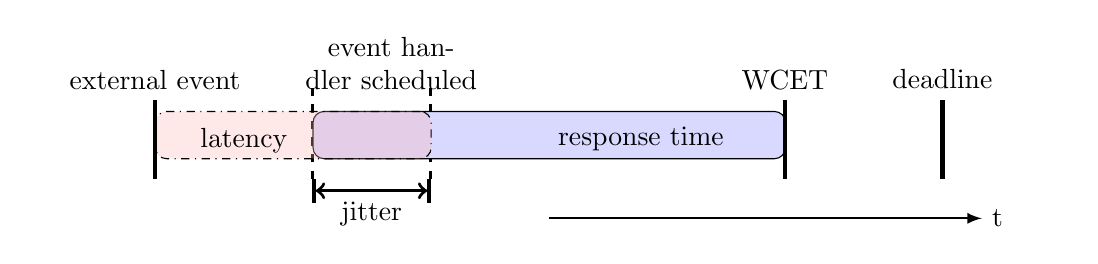
\begin{tikzpicture}
%\draw[gray, very thick, solid, >-<]  (0,1.5) -- (9,1.5) node at (4,1.5) [above] {relative deadline};
%\draw[black, very thick, ->]  (0,0) -- (10,0) node at (11,0) {time};
\draw[black, very thick, dashed] (2.0,0) -- (2.0,1.25) node at (3,1) [text width=3cm, above, align=center] {event handler scheduled};
\draw[black, very thick, dashed] (3.5,0) -- (3.5,1.25);

\node at (2.0,0.25)[rectangle, draw=black, fill=blue!15, rounded corners, minimum height = 0.6cm, minimum width = 6cm, anchor=south west] (resptime) {};

\begin{scope}[fill opacity=0.3]
\node at (0,0.25)[rectangle, draw=black, dashdotted, fill=red!30, rounded corners, minimum height = 0.6cm, minimum width = 3.50cm, anchor=south west] (latency) {};
%\node at (2.0,0.25)[rectangle, draw=black, postaction={pattern=north east lines}, minimum height = 0.6cm, minimum width = 1.5cm, anchor=south west] (overlap) {};
\end{scope}

\node [above left, inner sep=2pt] at (latency.south) {latency};
\node [above right, inner sep=3pt] at (resptime.south) {response time};

\draw[black, very thick, solid] (0,0) -- (0,1) node at (0,1) [text width=3cm, above, align=center] {external event};
\draw[black, very thick, solid] (8,0) -- (8,1) node at (8,1) [text width=3cm, above, align=center] {WCET};
\draw[black, ultra thick, solid] (10,0) -- (10,1) node at (10,1) [text width=3cm, above, align=center] {deadline};

\draw[black, very thick, solid, |<->|] (2.0,-0.15) -- (3.5,-0.15) node (jitter) at (2.75,-0.15) [below] {jitter};

%\node (latlabel) at (1,-1.0) {latency};
%\node (jitlabel) at (4,-1.0) {jitter};
%\node (rtlabel) at (8,-1.0) {response time};

\begin{scope}[>=latex]
	%\draw [thick, ->] (latlabel) to [bend right=45] (latency.center);
	%\draw [thick, ->] (rtlabel) to [bend left=45] (resptime.center);
    	%\draw [thick, ->] (jitlabel) to [bend left=45] (jitter.center);
	\draw[black, thick, ->] (5,-0.5) -- (10.5,-0.5) node [right] {t};
\end{scope}
\end{tikzpicture}
\end{center}
\ifreport
\caption{Real-time task interrupt latency and jitter}
\fi
\label{fig-latency-jitter}
\end{figure}


The interrupt or event handling latency is not a fixed parameter. 
The variance of interrupt latency depends on the current state of the system, 
e.g. if the system is executing a high priority task then observed release time of the event is delayed until execution of a high priority task finishes. 
The interrupt latency also depends on hardware overhead, which can vary when multiple interrupts arrive at the same time and hardware posts them one by one based on their priority.
Designers of a real-time system software are supposed to keep the event handling latency within certain bounds to respect timing constraints. 
The variance of interrupt latency is usually referred as jitter. Figure \ref{fig-latency-jitter} shows the relationship of interrupt latency and latency jitter with rest of parameters.

In contrast to desktop and server application, real-time applications are designed to have deterministic response times.
The general purpose computing tasks are optimized for average running time. 
While a real-time task is optimized to have deterministic response time even at the expense of increased average-case running time.
Performance of the real-time application is always evaluated based on worst-case execution times.
The difference leads to a separate class of operating systems called real-time operating systems (RTOS) specifically designed to have deterministic properties.
Characteristics of RTOS are described in the next section.


\section{Real-Time Operating Systems} \label{sec:rtos-and-types}
The operating system, or general purpose operating system (GPOS), is a piece of software that manages the resources of hardware platform and provides a nice abstraction to application software for using these resources \cite{Tanenbaum:2014:MOS:2655363}. The kernel-based design is a common design approach for GPOS. The OS implements two completely isolated workspaces: kernel-space and user-space. The OS layer that manages the hardware and provides services to userspace makes up the kernel-space.
The user application resides in userspace and use services provided by the OS kernel. In kernel-based OS design, typical services provided to userspace applications by OS kernel are process management, inter-process communication, time management, interrupt handling, process synchronization. 

A real-time application typically executes on top of a real-time operating system (RTOS). 
The RTOS has the same responsibilities as a general-purpose operating system, 
however, the resource management and scheduling policies are usually different to guarantee deterministic behavior and respect timing constraints of real-time tasks.
Various design approaches have been used to design RTOS.
Following sections briefly shed light on most common design approaches.

\subsection{Pure Real-time Operating Systems}
A large number of operating systems are designed exclusively for real-time applications.
Pure RTOS are typically designed to target single or a few similar real-time applications. 
For example Contiki RTOS \cite{Dunkels:2004:CLF:1032658.1034117} is designed specifically for wireless sensor nodes and it is optimized for small footprint and power efficiency.
Purposely built real-time operating systems come in many varieties: some are designed for small footprint suited for embedded devices, and some for safety-critical applications like control of a nuclear power plant.
Many RTOSs are designed for small devices that use micro-controllers whiteout MMU support and occupy memory in the order of few tens of kilobytes.
Examples from this class are Nucleus RTOS \cite{nucleus_rtos}, $\mu$C/OS-III \cite{micrium-rtos} and Contiki \cite{contiki-online}.
On the other hand RTOSs like VxWorks \cite{vxworks-rtos} support high-end processor families with MMU (x86, ARM, MIPS, and PowerPC). 
Often these RTOSs are rich in library content to support complex devices like graphical displays.
Most of real-time operating systems from this category are commercial and proprietary. 
However, there are some RTOS that are open-source.
FreeRTOS \cite{freertos} is an open-source RTOS that belongs to this category.

\subsection{Extensions to GPOS Kernels} \label{sec:rtos-ext-gpos}
One of the key aspects of general purpose OS is that they support a large number of devices and are very rich in library features. 
Open-source GPOS like Linux enjoys the fact that large group of people is continuously adding support for new features and support for devices.
Many real-time operating systems lack this feature because only a small group of people are maintaining the source code. 
Hence, another type of real-time operating systems available today is based on general purpose OS kernel.
A well-known example from this category is PREEMPT\_RT patch \cite{PREEMPT-RT}. 
The patchset once applied converts Linux kernel to a real-time kernel.
In order to convert a non real-time kernel to real-time, the PREEEMPT\_RT patchset adds preemption to non-preemptible parts.
The non-preemptible parts of the Linux kernel include interrupt handlers and critical sections.
Interrupt handlers are modified to run in process context. 
Critical sections that include spinlocks are modified to be preemptible by enabling interrupts.
Another key feature added by the patch is priority inheritance to avoid priority inversion.  

\subsection{Dual-Kernels}
Yet another approach used to convert GPOS to real-time OS is adding a small and thin real-time kernel that runs in parallel to GP kernel.
Once the GP kernel boots up the system, the real-time kernel takes over the control of the hardware resources.
The real-time applications use API interface and scheduling policies provided by the real-time kernel and the GP kernel runs as a low priority task.
This approach was first adopted in the design of RTLinux \cite{yodaiken1999rtlinux}, followed by RTAI \cite{RTAI} and Xenomai\cite{Xenomai}. 
One of the disadvantages of dual-kernel based RTOS is that there is no separation between real-time and the host kernel.

\subsection{Microkernel-based RTOS}
The microkernel design approach, unlike monolithic kernels, provide a minimalistic set of features necessary for the kernel space. 
The remaining services run as server like processes on top of microkernel and user applications use services when necessary.
The microkernel-based real-time operating systems design approach leverage the idea of microkernel to separate real-time kernel from general-purpose.
One of the examples of such an operating system is L4RTL \cite{mehnert2001rtlinux} which follows microkernel-based implementation to replace RTLinux\cite{yodaiken1999rtlinux}.

%\subsubsection{Library-based (kernel-less)}
%\subsubsection{Monolithic}
%\subsubsection{Exokernel-VirtualMachine}


\section{Virtualization} % of Real-time Applications}
Virtualization refers to creating and hosting multiple virtual machines on one hardware platform.
The piece of software that enables virtualization and manages virtual machines is called virtual machine monitor (VMM) or hypervisor.
A virtual machine is an environment created by the hypervisor to host an operating system with applications running on top called guests.
Virtualization technology enables concurrent execution of multiple guests on the same hardware as shown in Figure \ref{fig-virtualization}.
Virtualization is widely used in cloud computing and enterprise domains mainly for software consolidation to reduce hardware costs.
Virtualization is also used to enhance the security of the software system through isolation and encapsulation of virtual machines \cite{bazargan2012state}.
If an application running on one VM is compromised the hypervisor can secure rest of the VMs by blocking the VM on which compromised application is running.

\begin{figure}[!htb]
\begin{center}
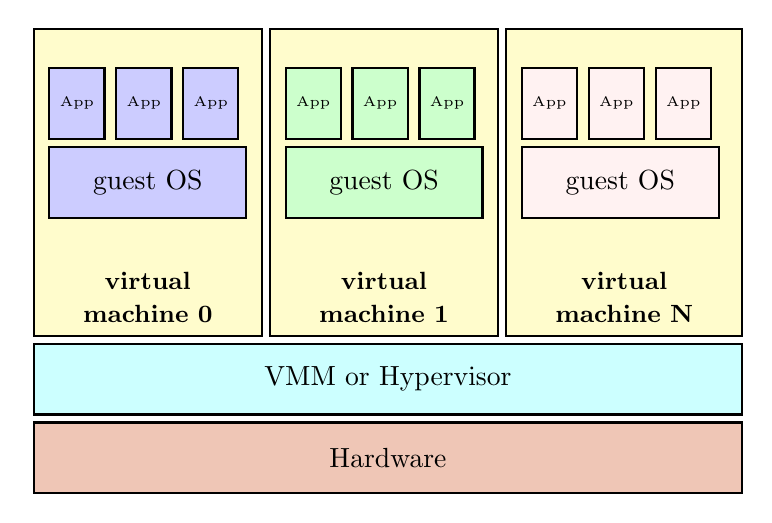
\begin{tikzpicture}

\node at (0,2) [rectangle, draw=black, thick, fill=yellow!20, minimum height = 3.9cm, minimum width = 2.9cm, anchor=south west] (vm0) {};
\node [above, inner sep=5pt, align=center, text width=2.7cm] at (vm0.south) {\textbf{\small{virtual\\ machine 0}}};

\node at (0.2,3.5) [rectangle, draw=black, thick, fill=blue!20, minimum height = 0.9cm, minimum width = 2.5cm, anchor=south west] (g0) {guest OS};
\node at (0.2,4.5) [rectangle, draw=black, thick, fill=blue!20, minimum height = 0.9cm, minimum width = 0.7cm, anchor=south west] (g0app0) {\tiny{App}};
\node at (0.2+0.85,4.5) [rectangle, draw=black, thick, fill=blue!20, minimum height = 0.9cm, minimum width = 0.7cm, anchor=south west] (g0app1) {\tiny{App}};
\node at (0.2+1.7,4.5) [rectangle, draw=black, thick, fill=blue!20, minimum height = 0.9cm, minimum width = 0.7cm, anchor=south west] (g0appn) {\tiny{App}};

\node at (3,2) [rectangle, draw=black, thick, fill=yellow!20, minimum height = 3.9cm, minimum width = 2.9cm, anchor=south west] (vm1) {};
\node [above, inner sep=5pt, align=center, text width=2.7cm] at (vm1.south) {\textbf{\small{virtual\\ machine 1}}};
\node at (3.2,3.5) [rectangle, draw=black, thick, fill=green!20, minimum height = 0.9cm, minimum width = 2.5cm, anchor=south west] (g1) {guest OS};
\node at (3.2,4.5) [rectangle, draw=black, thick, fill=green!20, minimum height = 0.9cm, minimum width = 0.7cm, anchor=south west] (g1app0) {\tiny{App}};
\node at (3.2+0.85,4.5) [rectangle, draw=black, thick, fill=green!20, minimum height = 0.9cm, minimum width = 0.7cm, anchor=south west] (g1app1) {\tiny{App}};
\node at (3.2+1.7,4.5) [rectangle, draw=black, thick, fill=green!20, minimum height = 0.9cm, minimum width = 0.7cm, anchor=south west] (g1appn) {\tiny{App}};

\node at (6,2) [rectangle, draw=black, thick, fill=yellow!20, minimum height = 3.9cm, minimum width = 3cm, anchor=south west] (vmn) {};
\node [above, inner sep=5pt, align=center, text width=2.7cm] at (vmn.south) {\textbf{\small{virtual\\ machine N}}};
\node at (6.2,3.5) [rectangle, draw=black, thick, fill=pink!20, minimum height = 0.9cm, minimum width = 2.5cm, anchor=south west] (gn) {guest OS};
\node at (6.2,4.5) [rectangle, draw=black, thick, fill=pink!20, minimum height = 0.9cm, minimum width = 0.7cm, anchor=south west] (gnapp0) {\tiny{App}};
\node at (6.2+0.85,4.5) [rectangle, draw=black, thick, fill=pink!20, minimum height = 0.9cm, minimum width = 0.7cm, anchor=south west] (gnapp1) {\tiny{App}};
\node at (6.2+1.7,4.5) [rectangle, draw=black, thick, fill=pink!20, minimum height = 0.9cm, minimum width = 0.7cm, anchor=south west] (gnappn) {\tiny{App}};

\node at (0,1) [rectangle, draw=black, thick, fill=Cyan!20, minimum height = 0.9cm, minimum width = 9cm, anchor=south west] (hyper) {VMM or Hypervisor};
\node at (0,0) [rectangle, draw=black, thick, fill=BrickRed!20, minimum height = 0.9cm, minimum width = 9cm, anchor=south west] (hard) {Hardware};


\end{tikzpicture}
\end{center}
\ifreport
\caption{Virtualization Technology}
\fi
\label{fig-virtualization}
\end{figure}


Virtualization has been around for decades. In 1972 IBM released VM/370 operating system for mainframe computers capable of running guest operating systems.
The hypervisors can be classified into two types.
Type-I hypervisor runs bare-metal and has full control over the hardware resources.
An example of type-I hypervisor is Xen \cite{Barham:2003:XAV:1165389.945462}.
Type-II hypervisor runs in a hosted environment on top of another operating system as a process.
An example of type-I hypervisor is KVM \cite{kivity2007kvm}.
The type-II hypervisor can only utilize resources allocated by the host operating system.
Type-I hypervisor can be more efficient than type-II, as it runs directly on the hardware.

\subsection{Virtualization Techniques}
Virtualization can be achieved in a number of ways. This section presents well-known techniques used for virtualization.

\subsubsection{Classical Virtualization}
In 1974, Popek and Golberg defined a virtual machine as \emph{"an efficient, isolated duplicate of the real machine"} and presented formal requirements to virtualize a computer architecture \cite{popek1974formal}. They described three most important characteristics of a virtual machine as follows:

\begin {itemize}
	\item {\textbf{Equivalence:}} The virtual environment provided to the virtual machine is essentially identical. The guest operating system can run in the virtual environment as if running on actual hardware.
	\item {\textbf{Performance:}} The virtual machine running in a virtual environment has comparable performance to when running natively.
	\item {\textbf{Resource Control:}} The virtual machine monitor software is in full control of all the system resources. The guest running in the virtual environment has access to only the resources explicitly allocated to this virtual machine.
\end {itemize}

These characteristics provided formal requirements for virtual machine monitor and underlying hardware architecture.
The virtual machine monitor provides duplicate execution environment to the real machine and does not add too much overhead to the execution of virtual machine.
Furthermore, virtual machine monitor has full control over hardware resources.

An instruction set architecture (ISA) of a CPU defines at least two privilege levels or modes of operation.
The set of instructions that can only be executed in highest privileged mode are called \emph{"privileged instructions"}.
Such instruction generates a fault if executed in user mode.
The highest privilege mode is used by operating system kernel to access and manage system resources.
User applications run in less privileged mode than the operating system kernel.
Popek and Golberg designated set of instruction that has different behavior depending on the mode of operation as \emph{"sensitive instructions"}.
These instructions included IO operations and instructions that interact with MMU.
Popek and Golberg stated that a computer architecture is virtualizable only if the set of sensitive instructions is a subset of privileged instructions. 
The computer architectures that fulfill Popek and Goldberg's criteria are called classically virtualizable architectures.
Classically virtualizable architectures can be used to implement faithful virtualization.
Faithful virtualization technique does not require modification in the guest operating system.

\begin{figure}[!htb]
\begin{center}
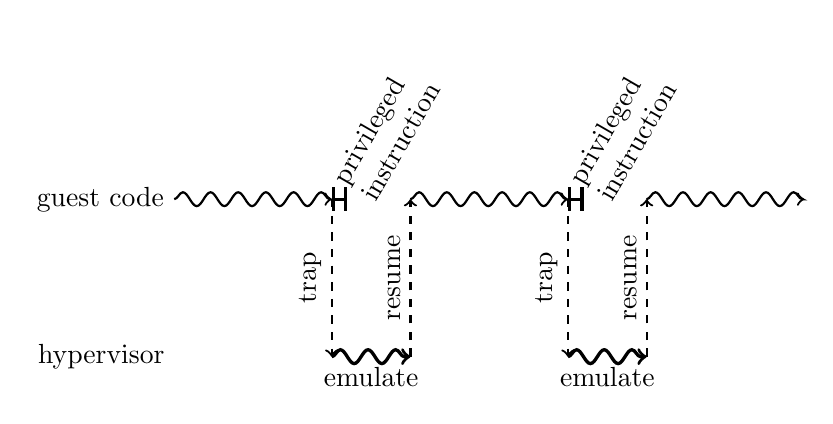
\begin{tikzpicture}


\draw[thick, decorate, decoration=snake, ->] (0, 2) -- (2, 2) node at (0,2) [left] {guest code};
\draw[very thick, |-|] (2, 2) -- (2.2, 2) node [above, right, rotate=60, text width=2cm]{privileged instruction};

\node at (0,0) [left] {hypervisor};
\draw[thick, dashed, ->] (2, 2) -- (2, 0) node [above, align=center,midway, rotate=90]{trap};
\draw[very thick, decorate, decoration=snake, ->] (2.0, 0) -- (3, 0) node [below,midway] {emulate};
\draw[thick, dashed, ->] (3, 0) -- (3, 2) node [above, align=center, midway, rotate=90] {resume};

\draw[thick, decorate, decoration=snake, ->] (3, 2) -- (5, 2);
\draw[very thick, |-|] (5, 2) -- (5.2, 2) node [above, right, rotate=60, text width=2cm]{privileged instruction};

\draw[thick, dashed, ->] (5, 2) -- (5, 0) node [above, align=center,midway, rotate=90]{trap};
\draw[very thick, decorate, decoration=snake, ->] (5, 0) -- (6, 0)  node [below,midway] {emulate};
\draw[thick, dashed, ->] (6, 0) -- (6, 2) node [above, align=center,midway, rotate=90]{resume};

\draw[thick, decorate, decoration=snake, ->] (6, 2) -- (8, 2);

\end{tikzpicture}
\end{center}
\ifreport
\caption{Faithful Virtualization (trap-and-emualte)}
\fi
\label{fig-virt-faithful}
\end{figure}


Faithful virtualization technique allows direct execution of most of the guest code. 
Hypervisor emulates parts of the guest code that cannot be executed directly on the hardware.
Faithful virtualization is achieved by executing guest code in a less privileged processor mode in which privileged instructions are not allowed to execute. 
When the processor encounters a privileged instruction it generates a fault, trapping into hypervisor code.
The hypervisor takes control and emulates the behavior of faulted guest operating system code. 
Once the required behavior is emulated, the guest code starts executing again directly on the CPU.
Figure \ref{fig-virt-faithful} demonstrates faithful virtualization technique.
The guest OS is fooled into believing that it is executing in highest privileged mode.  
This technique is also called trap-and-emulate as virtualization is achieved by emulating trapped guest OS code.   
Faithful virtualization achieves good performance as most of the guest code executes directly. 
%%Unlike paravirtualization in faithful virtualization the guest OS can execute without modification.
%%This technique is also called classical virtualization because the underlying cpu architecture has to satisfy Popek and Goberg requirement for virtualization.


\subsubsection{Software-based Virtualization}
Software-based virtualization technique translates guest operating system instructions into instruction of the target hardware.
This technique is also known as Emulation. 
In this technique effect of the guest is generated by emulating the behavior of the guest code. 
Figure \ref{fig-virt-software} demonstrates software-based virtualization technique.
One of the advantages of using emulation is that guest ISA and host ISA can be different. 
Emulation is useful in situations where target hardware is not accessible or very expensive to use. 
\begin{figure}[!htb]
\begin{center}
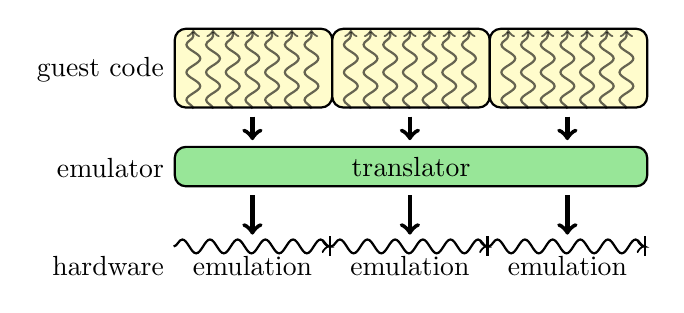
\begin{tikzpicture}

\node at (0,2.5) [left] {guest code};
\node at (0,2) [rectangle, draw=black, thick, rounded corners, fill=yellow!20,  minimum height = 1cm, minimum width = 2cm, anchor=south west] (b1) {};
\begin {scope} [opacity=0.6]
\draw[thick, decorate, decoration=snake, ->] (0.25, 2) -- (0.25, 3);
\draw[thick, decorate, decoration=snake, ->] (0.5, 2) -- (0.5, 3);
\draw[thick, decorate, decoration=snake, ->] (0.75, 2) -- (0.75, 3);
\draw[thick, decorate, decoration=snake, ->] (1, 2) -- (1, 3);
\draw[thick, decorate, decoration=snake, ->] (1.25, 2) -- (1.25, 3);
\draw[thick, decorate, decoration=snake, ->] (1.5, 2) -- (1.5, 3);
\draw[thick, decorate, decoration=snake, ->] (1.75, 2) -- (1.75, 3);
\end {scope}

\node at (2,2) [rectangle, draw=black, thick, rounded corners, fill=yellow!20, minimum height = 1cm, minimum width = 2cm, anchor=south west] (b2) {};
\begin {scope} [opacity=0.6]
\draw[thick, decorate, decoration=snake, ->] (2.25, 2) -- (2.25, 3);
\draw[thick, decorate, decoration=snake, ->] (2.5, 2) -- (2.5, 3);
\draw[thick, decorate, decoration=snake, ->] (2.75, 2) -- (2.75, 3);
\draw[thick, decorate, decoration=snake, ->] (3, 2) -- (3, 3);
\draw[thick, decorate, decoration=snake, ->] (3.25, 2) -- (3.25, 3);
\draw[thick, decorate, decoration=snake, ->] (3.5, 2) -- (3.5, 3);
\draw[thick, decorate, decoration=snake, ->] (3.75, 2) -- (3.75, 3);
\end {scope}

\node at (4,2) [rectangle, draw=black, thick, rounded corners, fill=yellow!20, minimum height = 1cm, minimum width = 2cm, anchor=south west] (b2) {};
\begin {scope} [opacity=0.6]
\draw[thick, decorate, decoration=snake, ->] (4.25, 2) -- (4.25, 3);
\draw[thick, decorate, decoration=snake, ->] (4.5, 2) -- (4.5, 3);
\draw[thick, decorate, decoration=snake, ->] (4.75, 2) -- (4.75, 3);
\draw[thick, decorate, decoration=snake, ->] (5, 2) -- (5, 3);
\draw[thick, decorate, decoration=snake, ->] (5.25, 2) -- (5.25, 3);
\draw[thick, decorate, decoration=snake, ->] (5.5, 2) -- (5.5, 3);
\draw[thick, decorate, decoration=snake, ->] (5.75, 2) -- (5.75, 3);
\end {scope}

\draw[ultra thick, ->] (1, 1.9) -- (1, 1.6);
\draw[ultra thick, ->] (3, 1.9) -- (3, 1.6);
\draw[ultra thick, ->] (5, 1.9) -- (5, 1.6);
\draw[ultra thick, ->] (1, 0.9) -- (1, 0.4);
\draw[ultra thick, ->] (3, 0.9) -- (3, 0.4);
\draw[ultra thick, ->] (5, 0.9) -- (5, 0.4);

\node at (0,1) [rectangle, draw=black, thick, rounded corners,  fill=LimeGreen!50, minimum height = 0.5cm, minimum width = 6cm, anchor=south west] (tr) {translator};
\node at (0,1.25) [left] {emulator};

\node at (0,0) [left] {hardware};
\draw[thick, decorate, decoration=snake, ->|] (0, 0.25) -- (2, 0.25)  node [below, align=center, midway, text width=2cm] {emulation};
\draw[thick, decorate, decoration=snake, ->|] (2, 0.25) -- (4, 0.25)  node [below, align=center, midway, text width=2cm] {emulation};
\draw[thick, decorate, decoration=snake, ->|] (4, 0.25) -- (6, 0.25)  node [below, align=center, midway, text width=2cm] {emulation};

\end{tikzpicture}
\end{center}
\ifreport
\caption{Software-based Virtualization}
\fi
\label{fig-virt-software}
\end{figure}


The performance of emulation is poor compared to other virtualization techniques where guest code can run directly on the target hardware. 
Techniques like dynamic binary translation and translation cache are used to improve the performance of an emulator \cite{ebcioglu2001dynamic}.
An example of virtualization software from this class is QEMU \cite{bellard2005qemu}.
QEMU is one of the most extensively used emulator, it uses optimization techniques like binary translation and translation cache to improve performance. 


\subsubsection{Paravirtualization}
Paravirtualization is a technique in which the hypervisor provides set of functions to the guest operating system to perform sensitive operations. 
The guest operating system is modified to replace the sensitive instructions with function calls, also referred as hypercalls.
The guest operating system software is executed directly on the hardware as long as no sensitive operation is required. 
Figure \ref{fig-virt-para} demonstrates paravirtualization technique.
A disadvantage of this technique is that guest OS has to be modified to replace sensitive operations.
\begin{figure}[!htb]
\begin{center}
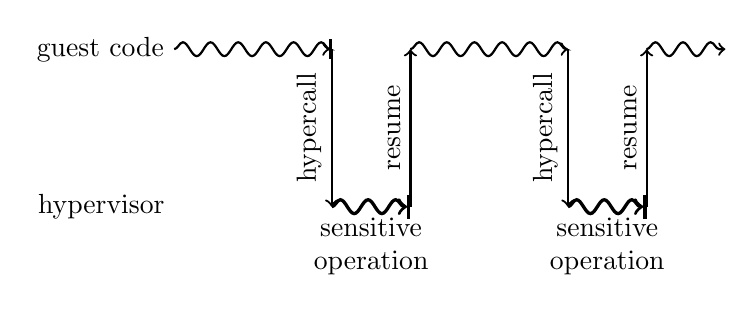
\begin{tikzpicture}


\draw[thick, decorate, decoration=snake, ->|] (0, 2) -- (2, 2) node at (0,2) [left] {guest code};
%\draw[thick, |-|] (2, 2) -- (2.3, 2) ; node [right, rotate=90, text width=2cm]{sensitive instruction};

\node at (0,0) [left] {hypervisor};
\draw[thick, ->] (2, 2) -- (2, 0) node [above, align=center,midway, rotate=90]{hypercall};
\draw[very thick, decorate, decoration=snake, ->|] (2.0, 0) -- (3, 0)   node [below, align=center, midway, text width=2cm] {sensitive operation};
\draw[thick, ->] (3, 0) -- (3, 2) node [above, align=center, midway, rotate=90] {resume};

\draw[thick, decorate, decoration=snake, ->] (3, 2) -- (5, 2);
%\draw[thick, |-|] (5, 2) -- (5.3, 2) node [right, rotate=90, text width=2cm]{sensitive operation};

\draw[thick, ->] (5, 2) -- (5, 0) node [above, align=center,midway, rotate=90]{hypercall};
\draw[very thick, decorate, decoration=snake, ->|] (5, 0) -- (6, 0)  node [below, align=center, midway, text width=2cm] {sensitive operation};
\draw[thick, ->] (6, 0) -- (6, 2) node [above, align=center,midway, rotate=90]{resume};

\draw[thick, decorate, decoration=snake, ->] (6, 2) -- (7, 2);

\end{tikzpicture}
\end{center}
\ifreport
\caption{Paravirtualization}
\fi
\label{fig-virt-para}
\end{figure}


The performance of paravirtualized guest OS is very close to executing guest operating system bare-metal.
An advantage of using paravirtualization over faithful virtualization is it can be used for architectures that lack hardware support for virtualization.
An example of this class is Xen hypervisor \cite{Barham:2003:XAV:1165389.945462}.
Xen is type-1 hypervisor that initially used paravirtualization to virtualize architectures that are not virtualizable. 
Xen also supports faithful virtualization through hardware-assisted virtualization.

\subsection{Virtualization of Real-time Applications}

Virtualization has been around for decades however the main area of deployment was usually desktop and server computers.
Since real-time system are subjected to strict timing constraints and require deterministic response times, any virtualization solution for real-time applications must address these issues.
Over the past few years, many virtualization solutions for real-time applications has been proposed.
Most virtualization solutions are customized to target one or a set of similar market segments of real-time systems. 
An example is Xtratum hypervisor which is specifically designed to host safety-critical applications \cite{Carrascosa:2014:XHR:2668138.2668142}.
Custom designed commercial virtualization solutions for real-time application also exist. 
Examples include WindRiver hypervisor for VxWorks \cite{bialowas2010achieving}, 
Greenhills INTEGRITY multivisor\cite{greenhills-multivisor}, 
Real-Time Systems GmbH Hypervisor \cite{realtime-systems-gmbh-hypervisor}
SysGO PikeOS \cite{kaiser2007pikeos}, 
and National Instruments Real-Time Hypervisor \cite{ni-realtime-hypervisor}.

Many researchers have focused on bringing real-time capabilities to widely used open-source virtualization software.
Xen \cite{Barham:2003:XAV:1165389.945462} is an open-source type-1 hypervisor widely used in research and cloud services.
A large amount of research has been conducted to make is acceptable for real-time applications.
Masrur et al. \cite{masrur2010vm} evaluated real-time performance of Xen SEDF (Simple Earliest Deadline First)
scheduling algorithm. They proposed PSEDF (Priority-based scheduling plus SEDF) that separates
real-time domains from other domains to achieve lower latencies and jitter.
RT-Xen project \cite{Xi:2011:RTR:2038642.2038651} has developed real-time scheduling framework for Xen.
Xen uses split-driver architecture for handling I/O. A special guest, called domain0, contains the
back-end driver and other guests (referred as user domains) contain front-end driver.
Physical interrupts are first delivered to the hypervisor. Hypervisor passes them to back-end drivers in domain0.
From domain0 they are routed to the front-end drivers in user domains.
Many research efforts have been made to lower interrupt response times caused by split-driver model.

KVM on the other hand is a type-2 hypervisor and uses Linux as host \cite{kivity2007kvm}. 
It is also an open-source project and extensively used in virtualization solution for the enterprise domain.
Kiszka \cite{kiszka2009towards} proposed real-time improvements to Linux host to append real-time capabilities to KVM.
One of the improvements was using PREEMPT\_RT patch to append real-time capabilities to host Linux kernel.
Zhang et al. \cite{zuo2010performance} proposed real-time virtualization solution based on KVM and suggested improvements to 
enhance real-time performance. The improvements include CPU shielding and interrupt prioritization. CPU shielding
refers to allocating a CPU core to real-time application. 

Many real-time virtualization solutions based on L4 microkernel has been proposed. 
In contrast to the monolithic kernel, a microkernel based design enjoys the benefit of having small TCB \cite{Heiser:2008:RVE:1435458.1435461}.
Examples include OKL4 microkernel-based hypervisor designed by Open Kernel Labs and PikeOS hypervisor developed by SysGo.
One application area for microkernel-based virtualization solutions is mobile platforms like smartphones.
The lightweight virtualization solution can enable co-existence of a GPOS for user interface applications and
RTOS to handle performance critical tasks.

%%Aavailability of large amounts of computational power on a single multicore chip and emerging technological trends has brought new opportunities and challenges for real-time systems.
%%Virtualization can be used to consolidate mixed criticality applications to efficiently use computational resources on multicore chip and reduced system costs.
%%Real-time systems are now accessible than ever before. Emerging technological trends has streered them to provide user access over the network.
%%Virtualization can provide security to real-time applications.
%%Many real-time applications run on a hetrogeneous computing platform with non real-time applications running aside. 
%%Virtualization can be used in such scenarios to isolated real-time applications from others.

\subsection{Virtual Machines on Multicore}
Multicore processors have become a norm and the average number of cores available per processors are expected to increase in future.
Multicore processing provides unique opportunities for real-time virtualization solutions.
Multicore processors have enabled co-location of applications of mixed-criticality on one platform by sandboxing each on the separate set of cores.
Although recent technological trends have increased the complexity of real-time applications, most real-time applications are relatively simpler than general-purpose applications.
Many software solutions include applications of mixed-criticality.
The availability of tremendous amounts of computing power on a multicore chip can be efficiently utilized if real-time
and general-purpose applications are hosted on the same processor chip. This can be achieved using virtualization technology.
The real-time applications can be assigned dedicated processor core(s) to ensure spatial isolation from general-purpose applications.
Virtualizations enables consolidation of application of mixed-criticality on one machine that reduces system cost.
Many virtualization solutions have been proposed that use separate CPU cores to isolate real-time applications
from others. Examples include Jailhouse \cite{jailhouse}, Quest-V \cite{West:2016:VSK:2966277.2935748} and Xtratum \cite {Carrascosa:2014:XHR:2668138.2668142} hypervisors.


\section{Hardware-Assisted Virtualization on x86}
For a long time, the x86 architecture was not virtualizable as it did not fulfill Popek and Goldberg's criteria.
Software-based emulation has remained the only choice of faithful virtualization for x86 architecture until 2005.
In the year 2005, Intel \cite{uhlig2005intel} and AMD released hardware extensions (VT-x and SVM respectively) that allowed x86 to be virtualized using the classical trap-and-emulate technique.
This section presents how hardware-assisted virtualization works.
The discussion is primarily based on Intel VT-x technology, however, it is equally valid for AMD SVM.

\subsection{Processor Operation Modes}

Intel Virtualization Technology (VT-x) adds virtual machine extensions (VMX) to the existing x86 architecture.
The technology defines two new modes of processor operation: VMX root operation mode and VMX non-root operation mode \cite{intel-sdm-vol3}.
The hypervisor runs in VMX root operation mode and the guest operating system executes in VMX non-root operation mode.
Both modes of operation include all privilege rings, which allows guest code to run at its intended ring. 
Hence no de-privileging is needed for the guest OS.

\begin{table}[h!]
\centering
\begin{tabular}{|r|c|c|} 
\hline
	\textbf{CPU operation mode}	&	{\textbf{VMX non-root}} 	&	{\textbf{VMX root}} \\ \hline \hline
	Instruction set		&	sensitive instructions 		&  new instruction added \\
                        &	are restricted (e.g. out	&  to manage VMs \\ 
                        &	instruction cause trap to   & (e.g. \mVMLAUNCH{},  \\ 
                        &	VMX root mode)              & \mVMREAD{}, \mVMWRITE{}) \\ \hline      		 	         
	Protection Rings	&	all (level0-3)	&	all (level0-3) \\ \hline
    Hardware Features   &   same            &  MMU, TLB, APIC \\ 
						&                   &  virtualization \\ \hline
	Software Stack		&	OS (Kernel and User)	&	Hypervisor \\ \hline
\end{tabular}
\caption{VT-x CPU modes of operation summary} 
\label{cpu-modes-summary}
\end{table}


VT-x technology defines two types of transition for VMX operation modes. 
Transitions into VMX non-root operation are called VM entries. 
Transitions from VMX non-root to VMX root operation mode are called VM exits.
In VMX root operation mode processor functionality is extended with new instruction set that
the hypervisor can use to create and manage virtual machines.
The functionality of VMX non-root operation is restricted. 
Execution of a sensitive instruction can cause VM exit giving control back to the hypervisor.
Once a virtual machine is properly configured by the hypervisor, these modes of operation are hidden from the guest. 
Table \ref{cpu-modes-summary} summarizes the new modes of operation support by VT-x.


\subsection{Virtual Machine Control Structure}
VT-x technology allows configuration and management of a virtual machine via data structure called virtual machine control structure (VMCS).
The hypervisor can control the behavior of virtual CPU by properly configuring VMCS data structure.
The hypervisor is responsible to allocate, initialize and manage one VMCS data structure for each virtual processor.
The VMCS is further divided into subfields as follows:
\begin{itemize}
	\item \textbf{Guest-state area} used to load and store guest state on vmx transitions
	\item \textbf{Host-state area} used to load and store host state on vmx transitions
	\item \textbf{VM-execution control fields} includes fields to controls vmx non-root operation mode
	\item \textbf{VM-exit control fields} includes fields to controls vmexit transition
	\item \textbf{VM-entry control fields} includes fields to control vmentry transition
	\item \textbf{VM-exit information fields} used to store information about vmexit transition
\end{itemize}

VT-x technology supports new instructions that hypervisor can use in VMX root operating mode to manage VMCS.
For example, to read and write a field of VMCS host uses \mVMREAD{} and \mVMWRITE{} instruction respectively.

\begin{figure}[!htb]
\begin{center}
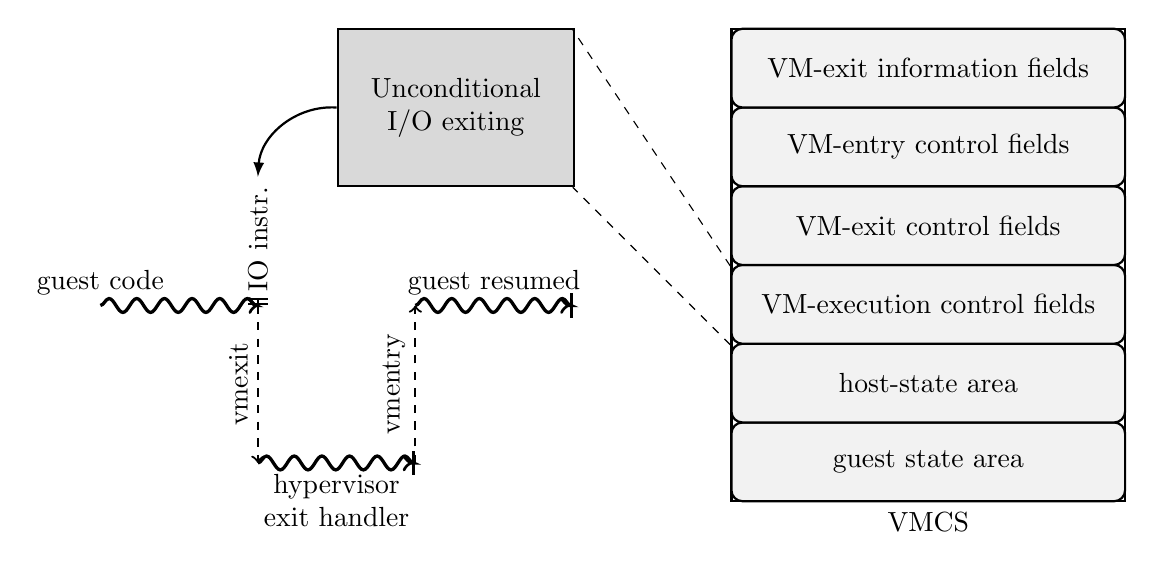
\begin{tikzpicture}

%\draw[step=0.5cm, gray, very thin] (0,0) grid (9,9)


\draw[very thick, decorate, decoration=snake, ->] (0, 2.5) -- (2, 2.5) node at (0,2.5) [above] {guest code};
\draw[thick, |-|] (2, 2.5) -- (2, 2.6) node at (2, 2.6)[right, midway, rotate=90] (ioinst) {IO instr.};

\draw[very thick, decorate, decoration=snake, ->|] (2, 0.5) -- (4, 0.5) node [below, midway, align=center] {hypervisor\\ exit handler};
\draw[very thick, decorate, decoration=snake, ->|] (4, 2.5) -- (6, 2.5) node [above, align=center, midway] {guest resumed};

\draw[thick, dashed, ->] (2, 2.5) -- (2, 0.5) node [above, align=center,midway, rotate=90] {vmexit};
\draw[thick, dashed, ->] (4, 0.5) -- (4, 2.5) node [above, align=center,midway, rotate=90] {vmentry};


\node at (3,4) [rectangle, draw=black, thick, fill=black!15, minimum height = 2cm, minimum width = 3cm, anchor=south west, align=center] (exitcontrol) 
                        {Unconditional\\ I/O exiting} ;


\node at (8,0) [rectangle, draw=black, thick, fill=white, minimum height = 6cm, minimum width = 5cm, anchor=south west] (vmcs) {} ;
\node [below, align=center] at (vmcs.south) {VMCS};
%\node[below right, inner sep=5pt, text width=2cm] at (rtguest.north west) {PREEMPT\_RT\\ Linux\\ (rt-guest)};


\node at (8,0) [rectangle, draw=black, thick, rounded corners, fill=black!5, minimum height = 1cm, minimum width = 5cm, anchor=south west] (gstate) {guest state area};
\node at (8,1) [rectangle, draw=black, thick, rounded corners, fill=black!5, minimum height = 1cm, minimum width = 5cm, anchor=south west] (gstate) {host-state area};
\node at (8,2) [rectangle, draw=black, thick, rounded corners, fill=black!5, minimum height = 1cm, minimum width = 5cm, anchor=south west] (gstate) {VM-execution control fields};
\node at (8,3) [rectangle, draw=black, thick, rounded corners, fill=black!5, minimum height = 1cm, minimum width = 5cm, anchor=south west] (gstate) {VM-exit control fields};
\node at (8,4) [rectangle, draw=black, thick, rounded corners, fill=black!5, minimum height = 1cm, minimum width = 5cm, anchor=south west] (gstate) {VM-entry control fields};
\node at (8,5) [rectangle, draw=black, thick, rounded corners, fill=black!5, minimum height = 1cm, minimum width = 5cm, anchor=south west] (gstate) {VM-exit information fields};

\draw [dashed] (8,2) -- (6,4); 
\draw [dashed] (8,3) -- (6,6); 

\begin{scope}[>=latex]
	\draw [thick, ->] (exitcontrol.west) to [bend right=45] (ioinst.east);
\end{scope}

\end{tikzpicture}
\end{center}
\ifreport
\caption{VMCS data structure with an example of using VMCS fields to control guest execution behavior}
\fi
\label{fig-vmcs-ds}
\end{figure}


\subsection{Virtual Machine Control Flow}
The hypervisor enters VMX root operation mode by executing \mVMXON{} instruction.
The \mVMLAUNCH{} instruction is used to launch a virtual machine that causes VM entry.
On VM entry transition hardware loads guest state from the guest-state area of VMCS
and begins execution of guest code at an address specified in VMCS.
During VM entry transition the hardware checks fields of VMCS to 
identify if hypervisor has request injection of a virtual interrupt.
If so, the virtual interrupt is delivered to the guest right after VM entry transition.
Flags in VMCS VM-execution control fields area define when to take VM exit transition.
For example \emph{"Unconditional IO exiting"} flag will cause VM exit transition 
when guest code tries to execute an IO instruction. Figure \ref{fig-vmcs-ds} demonstrates 
what happens when IO instruction is encountered in guest code.
Similarly, \emph{"external interrupt exiting"} will cause VM exit transition if
an external interrupt arrives in vmx non-root operation mode, giving control back to the hypervisor.
During VM exit transition the hardware stores guest state back to the guest-state area in VMCS and
loads host state from the host-state area in VMCS.
Furthermore, the detailed information about the cause of VM exit transition is
saved in VM-exit information area in VMCS. This information helps hypervisor
to determine appropriate action required to emulate the guest behavior.

\subsection{Features for Efficient Virtualization}
This section sheds light upon x86 hardware features that enable efficient virtualization of guests.

\subsubsection{MMU Virtualization} \label{sec:vmmu}
In a virtualized environment a guest executes in its own virtual address space and hypervisor has full control over the physical memory.
In order to keep the illusion that guest has control over physical memory, hypervisor uses nested page-tables also known as shadow page-tables.
When a guest tries to access physical memory, guest physical addresses are treated as virtual addresses and 
translated to real physical addresses through nested page-tables.
The nested page-tables can be implemented in software in which case software emulates the behavior of page-table walk to
translate guest physical address (host virtual address) to host physical addresses.

\begin{figure}[!htb]
\begin{center}
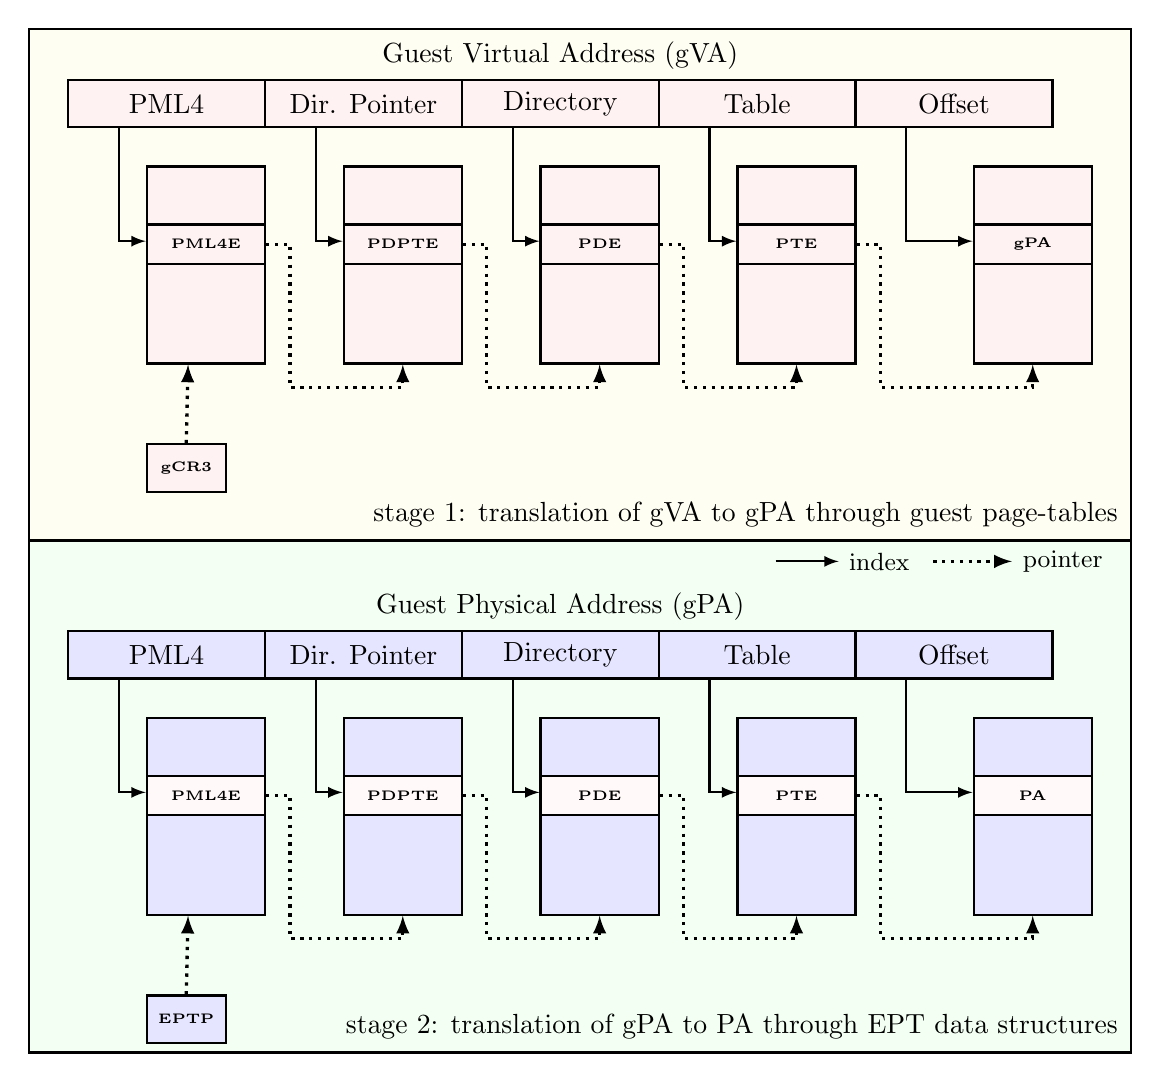
\begin{tikzpicture}

\node at (-0.5,-5-0.25) [rectangle, draw=black, thick, fill=yellow!5, minimum height = 6.5cm, minimum width = 14cm, anchor=south west] (stage1) {};
\node [above left, inner sep=5pt] at (stage1.south east) {\textbf\small{{stage 1: translation of gVA to gPA through guest page-tables}}};

\node at (0,0) [rectangle, draw=black, thick, fill=pink!20, minimum height = 0.6cm, minimum width = 2.5cm, anchor=south west] (gpml4) {PML4};
\node at (0+2.5,0) [rectangle, draw=black, thick, fill=pink!20, minimum height = 0.6cm, minimum width = 2.5cm, anchor=south west] (gdirptr) {Dir. Pointer};
\node at (0+2.5+2.5,0) [rectangle, draw=black, thick, fill=pink!20, minimum height = 0.6cm, minimum width = 2.5cm, anchor=south west] (gdir) {Directory};
\node [above, align=center] at (gdir.north) {\textbf\small{{Guest Virtual Address (gVA)}}};
\node at (0+2.5+2.5+2.5,0) [rectangle, draw=black, thick, fill=pink!20, minimum height = 0.6cm, minimum width = 2.5cm, anchor=south west] (gtbl) {Table};
\node at (0+2.5+2.5+2.5+2.5,0) [rectangle, draw=black, thick, fill=pink!20, minimum height = 0.6cm, minimum width = 2.5cm, anchor=south west] (goff) {Offset};


\node at (1.0,-3) [rectangle, draw=black, thick, fill=pink!20, minimum height = 2.5cm, minimum width = 1.5cm, anchor=south west] (gpgpml4) {};
\node [rectangle, draw=black, thick, fill=pink!20, minimum height = 0.5cm, minimum width = 1.5cm, anchor=south west] at (gpgpml4.west) (gpgpml4e) 
				{\tiny\textbf{{PML4E}}};

\node at (1.0,-4)  [rectangle, draw=black, thick, fill=pink!20, minimum height = 0.6cm, minimum width = 1.0cm, anchor=north west] (gcr3) 
				{\tiny\textbf{{gCR3}}};

\node at (3.5,-3) [rectangle, draw=black, thick, fill=pink!20, minimum height = 2.5cm, minimum width = 1.5cm, anchor=south west] (gpgdirptr) {};
\node [rectangle, draw=black, thick, fill=pink!20, minimum height = 0.5cm, minimum width = 1.5cm, anchor=south west] at (gpgdirptr.west) 
			    (gpgdirptre) {\tiny\textbf{{PDPTE}}};
\node at (6,-3) [rectangle, draw=black, thick, fill=pink!20, minimum height = 2.5cm, minimum width = 1.5cm, anchor=south west] (gpgdir) {};
\node [rectangle, draw=black, thick, fill=pink!20, minimum height = 0.5cm, minimum width = 1.5cm, anchor=south west] at (gpgdir.west) 
                (gpgdire) {\tiny\textbf{{PDE}}};
\node at (8.5,-3) [rectangle, draw=black, thick, fill=pink!20, minimum height = 2.5cm, minimum width = 1.5cm, anchor=south west] (gpgtbl) {};
\node [rectangle, draw=black, thick, fill=pink!20, minimum height = 0.5cm, minimum width = 1.5cm, anchor=south west] at (gpgtbl.west) 
                (gpgtble) {\tiny\textbf{{PTE}}};
\node at (11.5,-3) [rectangle, draw=black, thick, fill=pink!20, minimum height = 2.5cm, minimum width = 1.5cm, anchor=south west] (gpgoff) {};
\node [rectangle, draw=black, thick, fill=pink!20, minimum height = 0.5cm, minimum width = 1.5cm, anchor=south west] at (gpgoff.west) 
                {\tiny\textbf{{gPA}}};


\begin{scope}[>=latex]	
	\draw [thick, ->] ([xshift=-4ex]gpml4.south) |- ([yshift=2ex]gpgpml4.west);
	\draw [thick, ->] ([xshift=-4ex]gdirptr.south) |- ([yshift=2ex]gpgdirptr.west);
	\draw [thick, ->] ([xshift=-4ex]gdir.south) |- ([yshift=2ex]gpgdir.west);
	\draw [thick, ->] ([xshift=-4ex]gtbl.south) |- ([yshift=2ex]gpgtbl.west);
	\draw [thick, ->] ([xshift=-4ex]goff.south) |- ([yshift=2ex]gpgoff.west);

	%\draw [thick, dotted, ->] ([yshift=-1ex]gpgpml4e.south) to [bend right=75] (gpgdirptr.south);

	\draw [very thick, dotted, ->] (gcr3.north) -- ([xshift=-1.5ex]gpgpml4.south);
	\draw [very thick, dotted, ->] (gpgpml4e.east) -| ([xshift=2ex]gpgpml4e.east) -- ([xshift=2ex, yshift=-12ex]gpgpml4e.east) -| (gpgdirptr.south);
	\draw [very thick, dotted, ->] (gpgdirptre.east) -| ([xshift=2ex]gpgdirptre.east) -- ([xshift=2ex, yshift=-12ex]gpgdirptre.east) -| (gpgdir.south);
	\draw [very thick, dotted, ->] (gpgdire.east) -| ([xshift=2ex]gpgdire.east) -- ([xshift=2ex, yshift=-12ex]gpgdire.east) -| (gpgtbl.south);
	\draw [very thick, dotted, ->] (gpgtble.east) -| ([xshift=2ex]gpgtble.east) -- ([xshift=2ex, yshift=-12ex]gpgtble.east) -| (gpgoff.south);	

\end{scope}

\node at (-0.5,-5-7+0.25) [rectangle, draw=black, thick, fill=green!5, minimum height = 6.5cm, minimum width = 14cm, anchor=south west] (stage2) {};
\node [above left, inner sep=5pt] at (stage2.south east) {\textbf\small{{stage 2: translation of gPA to PA through EPT data structures}}};

\node at (0,0-7) [rectangle, draw=black, thick, fill=blue!10, minimum height = 0.6cm, minimum width = 2.5cm, anchor=south west] (gpml4) {PML4};
\node at (0+2.5,0-7) [rectangle, draw=black, thick, fill=blue!10, minimum height = 0.6cm, minimum width = 2.5cm, anchor=south west] (gdirptr) {Dir. Pointer};
\node at (0+2.5+2.5,0-7) [rectangle, draw=black, thick, fill=blue!10, minimum height = 0.6cm, minimum width = 2.5cm, anchor=south west] (gdir) {Directory};
\node [above, align=center] at (gdir.north) {\textbf\small{{Guest Physical Address (gPA)}}};
\node at (0+2.5+2.5+2.5,0-7) [rectangle, draw=black, thick, fill=blue!10, minimum height = 0.6cm, minimum width = 2.5cm, anchor=south west] (gtbl) {Table};
\node at (0+2.5+2.5+2.5+2.5,0-7) [rectangle, draw=black, thick, fill=blue!10, minimum height = 0.6cm, minimum width = 2.5cm, anchor=south west] (goff) {Offset};


\node at (1.0,-3-7) [rectangle, draw=black, thick, fill=blue!10, minimum height = 2.5cm, minimum width = 1.5cm, anchor=south west] (gpgpml4) {};
\node [rectangle, draw=black, thick, fill=pink!10, minimum height = 0.5cm, minimum width = 1.5cm, anchor=south west] at (gpgpml4.west) (gpgpml4e) 
				{\tiny\textbf{{PML4E}}};

\node at (1.0,-4-7)  [rectangle, draw=black, thick, fill=blue!10, minimum height = 0.6cm, minimum width = 1.0cm, anchor=north west] (eptp) 
				{\tiny\textbf{{EPTP}}};

\node at (3.5,-3-7) [rectangle, draw=black, thick, fill=blue!10, minimum height = 2.5cm, minimum width = 1.5cm, anchor=south west] (gpgdirptr) {};
\node [rectangle, draw=black, thick, fill=pink!10, minimum height = 0.5cm, minimum width = 1.5cm, anchor=south west] at (gpgdirptr.west) 
			    (gpgdirptre) {\tiny\textbf{{PDPTE}}};
\node at (6,-3-7) [rectangle, draw=black, thick, fill=blue!10, minimum height = 2.5cm, minimum width = 1.5cm, anchor=south west] (gpgdir) {};
\node [rectangle, draw=black, thick, fill=pink!10, minimum height = 0.5cm, minimum width = 1.5cm, anchor=south west] at (gpgdir.west) 
                (gpgdire) {\tiny\textbf{{PDE}}};
\node at (8.5,-3-7) [rectangle, draw=black, thick, fill=blue!10, minimum height = 2.5cm, minimum width = 1.5cm, anchor=south west] (gpgtbl) {};
\node [rectangle, draw=black, thick, fill=pink!10, minimum height = 0.5cm, minimum width = 1.5cm, anchor=south west] at (gpgtbl.west) 
                (gpgtble) {\tiny\textbf{{PTE}}};
\node at (11.5,-3-7) [rectangle, draw=black, thick, fill=blue!10, minimum height = 2.5cm, minimum width = 1.5cm, anchor=south west] (gpgoff) {};
\node [rectangle, draw=black, thick, fill=pink!10, minimum height = 0.5cm, minimum width = 1.5cm, anchor=south west] at (gpgoff.west) 
                {\tiny\textbf{{PA}}};

\begin{scope}[>=latex]	
	\draw [thick, ->] ([xshift=-4ex]gpml4.south) |- ([yshift=2ex]gpgpml4.west);
	\draw [thick, ->] ([xshift=-4ex]gdirptr.south) |- ([yshift=2ex]gpgdirptr.west);
	\draw [thick, ->] ([xshift=-4ex]gdir.south) |- ([yshift=2ex]gpgdir.west);
	\draw [thick, ->] ([xshift=-4ex]gtbl.south) |- ([yshift=2ex]gpgtbl.west);
	\draw [thick, ->] ([xshift=-4ex]goff.south) |- ([yshift=2ex]gpgoff.west);

	\draw [very thick, dotted, ->] (eptp.north) -- ([xshift=-1.5ex]gpgpml4.south);
	\draw [very thick, dotted, ->] (gpgpml4e.east) -| ([xshift=2ex]gpgpml4e.east) -- ([xshift=2ex, yshift=-12ex]gpgpml4e.east) -| (gpgdirptr.south);
	\draw [very thick, dotted, ->] (gpgdirptre.east) -| ([xshift=2ex]gpgdirptre.east) -- ([xshift=2ex, yshift=-12ex]gpgdirptre.east) -| (gpgdir.south);
	\draw [very thick, dotted, ->] (gpgdire.east) -| ([xshift=2ex]gpgdire.east) -- ([xshift=2ex, yshift=-12ex]gpgdire.east) -| (gpgtbl.south);
	\draw [very thick, dotted, ->] (gpgtble.east) -| ([xshift=2ex]gpgtble.east) -- ([xshift=2ex, yshift=-12ex]gpgtble.east) -| (gpgoff.south);	

	\draw [very thick, dotted, ->] (11,-5.5) -- (12, -5.5) node [right] {\small{pointer}};
	\draw [thick, ->] (9,-5.5) -- (9.8, -5.5) node [right] {\small{index}};
\end{scope}

\end{tikzpicture}
\end{center}
\ifreport
\caption{MMU Virtualization (inspired from \cite{West:2016:VSK:2966277.2935748})}
\fi
\label{fig-vmmu}
\end{figure}


Recent revisions of hardware-assisted virtualization extensions of x86 support translation of the guest physical address to host physical address
in hardware using a feature called extended page-tables (EPT) \cite{intel-sdm-vol3}.
The feature removes the need of maintaining nested page-tables in software, hence reducing software overhead to perform the translation.
Figure \ref{fig-vmmu} shows how the guest virtual address is translated to machine physical address using EPT data structures.
The first stage is the same, the guest virtual address is translated to guest physical address by using guest page-tables.
Then in stage 2, the guest physical address translated using extended page-tables in hardware. 
The translation processor is autonomous.

VT-x extensions also added the concept of virtual-processor identifiers (VPIDs). 
The feature allows processor the cache address translation of multiple address spaces by associated different VPIDs to each address space.
VPID is a 16-bit identifier, and the value 0 is reserved for the hypervisor.
The hypervisor assigns a unique VPID to each guest during virtual machine initialization.
This feature also allows VPID based TLB flushing and clearing single translations.
Table \ref{vpid-entries} shows the two types of TLB entries supported by VT-x extensions.

\begin{table}[!h]
\centering
\begin{tabular}{|c||c|c|c|}  
\hline
	\textbf{TLB Entry}	&	\textbf{VPID}	&	\textbf{Tag} &	\textbf{Data}\\ \hline \hline
	Guest			&	x $(x > 0)$		&		gVA 	 & 	gPA			 \\ \hline
	Hypervisor		&	0				&		VA 		 &  PA			 \\ \hline
\end{tabular}
\caption{TLB Partitioning, VPIDs allow hypervisor to separate address translations of the guests from each other and from the hypervisor} 
\label{vpid-entries}
\end{table}


\subsubsection{APIC Virtualization} \label{sec:vapic}
The x86 virtualization extensions VT-x supports virtualization of Local APIC (Advanced Programmable Interrupt Controller) \cite{intel-sdm-vol3}. 
The APIC virtualization (APIC-v) allows emulation of most interrupt controller register accesses by the guest and keeps track of the virtual APIC state. 
APIC-v supports direct injection of the virtual interrupts without hypervisor intervention through a feature called posted interrupts (PI).
The feature requires hypervisor to allocate a memory page for the guest where the virtual state of the APIC is maintained by the hardware.
All read accesses to the APIC registers are emulated in hardware by writing contents of virtual APIC memory page without hypervisor intervention.
The write accesses to APIC registers are also emulated in hardware by writing new values to virtual APIC page. 
However, for certain registers hypervisor intervention is required and the control is transferred to hypervisor at end of write emulation.
Figure \ref{fig-vapic} displays how virtual APIC page is accessed by the guest without hypervisor involvement. 
The hypervisor is responsible to allocate virtual APIC page and store address of the page in VMCS before initializing a virtual machine.
From there onwards, all access to APIC by the guest are virtualized by hardware.

\begin{figure}[!htb]
\begin{center}
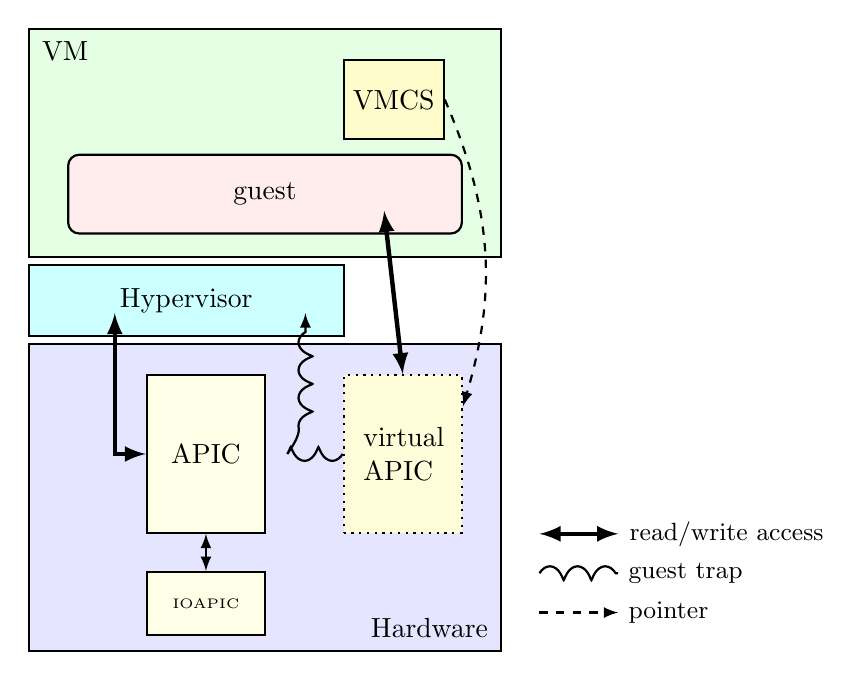
\begin{tikzpicture}

\node at (0,5) [rectangle, draw=black, thick, fill=green!10, minimum height = 2.9cm, minimum width = 6cm, anchor=south west] (vm) {};
\node [below right, inner sep=5pt] at (vm.north west) {VM};

\node at (0.5,5.3) [rectangle, rounded corners, draw=black, thick, fill=pink!30, minimum height = 1cm, minimum width = 5cm, anchor=south west] (g) {guest};
\node at (4.0,6.5) [rectangle, draw=black, thick, fill=yellow!20, minimum height = 1cm, minimum width = 0.5cm, anchor=south west] (vmcs) {VMCS};

\node at (0,4) [rectangle, draw=black, thick, fill=Cyan!20, minimum height = 0.9cm, minimum width = 4cm, anchor=south west] (hyper) {Hypervisor};

\node at (0,0) [rectangle, draw=black, thick, fill=blue!10, minimum height = 3.9cm, minimum width = 6cm, anchor=south west] (hard) {};
\node [above left, inner sep=5pt] at (hard.south east) {Hardware};

\node at (1.5,1.5) [rectangle, draw=black, thick, fill=yellow!10, minimum height = 2cm, minimum width = 1.5cm, anchor=south west] (apic) {APIC};
\node at (1.5,0.2) [rectangle, draw=black, thick, fill=yellow!10, minimum height = 0.8cm, minimum width = 1.5cm, anchor=south west] (ioapic) {\tiny{IOAPIC}};

\node at (4,1.5) [dotted, rectangle, draw=black, thick, fill=yellow!15, minimum height = 2cm, minimum width = 1.5cm, anchor=south west, text width=1cm] (vapic) {virtual APIC};

\begin{scope}[>=latex]	
	\draw [ultra thick, <->] (apic.west) -| ([xshift=-6ex, yshift=2ex]hyper.south) ;
	\draw [ultra thick, <->] ([xshift=10ex, yshift=2ex]g.south) -- (vapic.north) ;
	\draw [thick,  decorate, decoration=coil, ->] (vapic.west) -| ([xshift=10ex, yshift=2ex]hyper.south) ;
	\draw [thick, dashed, ->] (vmcs.east) to [bend left=20] ([yshift=4ex]vapic.east) ;
	\draw [thick, <->] (apic.south) -- (ioapic.north) ;

	\draw [ultra thick, <->] (6.5,1.5) -- (7.5,1.5) node [right] {\small{read/write access}};
	\draw [thick, decorate, decoration=coil] (6.5,1) -- (7.5,1) node [right] {\small{guest trap}};
	\draw [thick, dashed, ->] (6.5,0.5) -- (7.5,0.5) node [right] {\small{pointer}};
\end{scope}



\end{tikzpicture}
\end{center}
\ifreport
\caption{APIC Virtualization}
\fi
\label{fig-vapic}
\end{figure}


\subsubsection{Direct Interrupt Injection} \label{sec:dii}
Intel APIC-v feature enables direct injection of a virtual interrupt to the guest without intervention from the hypervisor.
Intel calls this feature Posted Interrupts (PI) Processing \cite{intel-sdm-vol3}. The mechanism uses a data structure called Posted Interrupt Descriptor (PID).
The PID contains bit-fields for to enable posted interrupt mechanism on the basis of the interrupt vector.
Figure \ref{fig-pi-ds} shows fields of PID data structure.
\begin{figure}[!htb]
\begin{center}
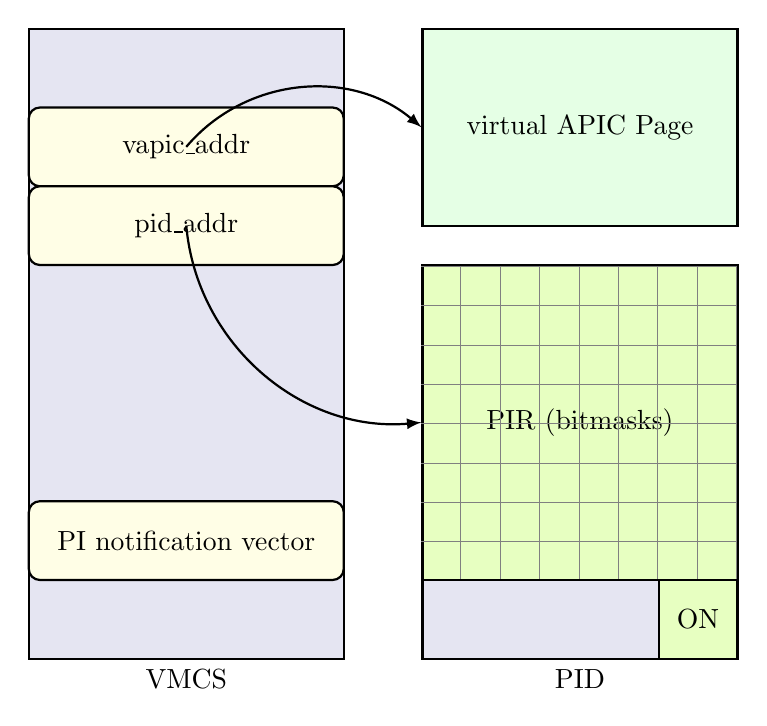
\begin{tikzpicture}


%%\draw[step=0.5cm, gray, very thin] (0,0) grid (9,9);

\node at (0,0) [rectangle, draw=black, thick, fill=NavyBlue!10, minimum height = 8cm, minimum width = 4cm, anchor=south west] (vmcs) {} ;
\node [below, align=center] at (vmcs.south) {VMCS};

\node at (0,6) [rectangle, draw=black, thick, fill=yellow!10, rounded corners, minimum height = 1cm, minimum width = 4cm, anchor=south west] (apicaddr)  {vapic\_addr};
\node at (0,5) [rectangle, draw=black, thick, fill=yellow!10, rounded corners, minimum height = 1cm, minimum width = 4cm, anchor=south west] (pidaddr)  {pid\_addr};

\node at (0,1) [rectangle, draw=black, thick, fill=yellow!10, rounded corners, minimum height = 1cm, minimum width = 4cm, anchor=south west] (pinv)  {PI notification vector};

\node at (5,1) [rectangle, draw=black, thick, fill=GreenYellow!30, minimum height = 4cm, minimum width = 4cm, anchor=south west] (pir) {PIR (bitmasks)};
\begin{scope}[fill opacity=0.9]
	\draw[xstep=0.5cm, ystep=0.5, gray, very thin] (5,1) grid (9,5);
\end{scope}

\node at (5,0) [rectangle, draw=black, thick, fill=NavyBlue!10, minimum height = 1cm, minimum width = 4cm, anchor=south west] (rsrvd) {};
\node at (8,0) [rectangle, draw=black, thick, fill=GreenYellow!30, minimum height = 1cm, minimum width = 1cm, anchor=south west] (on) {ON};
\node [below, align=center] at (rsrvd.south) {PID};

\node at (5,5.5) [rectangle, draw=black, thick, fill=green!10, minimum height = 2.5cm, minimum width = 4cm, anchor=south west] (vapic) {virtual APIC Page};


\begin{scope}[>=latex]
	\draw [thick, ->] (apicaddr.center) to [bend left=45] (vapic.west);
	\draw [thick, ->] (pidaddr.center) to [bend right=45] (pir.west);
\end{scope}


\end{tikzpicture}
\end{center}
\ifreport
\caption{Key data structures for Posted Interrupt processing. Virtual APIC page is used by VT-x to virtualize interrupt controller memory accesses. 
PINV is the interrupt vector number that uses PID data structure for delivery without exit.
PID consists of an ON bit and PIR bitmasks. Host marks PIR bit corresponding to interrupt vector and sets the ON bit
to deliver interrupt directly to the guest.}
\fi
\label{fig-pi-ds}
\end{figure}

PID is a field of VMCS and initialized by the host to inject interrupts owned by guest OS. 
The host also initializes posted interrupt notification vector (PINV) field in VMCS.
PINV is compared in hardware with the physical vector number to decide when an interrupt should be injected directly to the guest.
When an external interrupt whose physical vector is same as PINV arrives and PIR bit for the corresponding vector is set along with outstanding notification (ON) bit the interrupt is delivered to the guest without VM exit transition.
The direct interrupt injection allows reducing virtualization overhead. It enables the host to deliver interrupts from devices owned by the guest directly without
intervention. Figure \ref{fig-pi-delivery} shows how virtualization overhead can be reduced by direct interrupt injection mechanism.

\begin{figure}[!htb]
\begin{center}
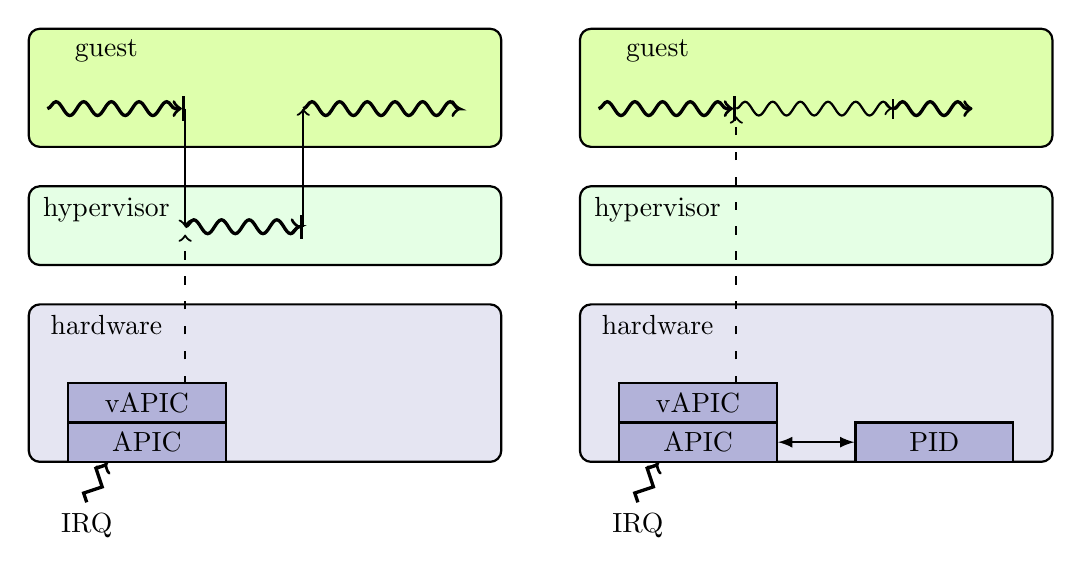
\begin{tikzpicture}


%\draw[step=0.5cm, gray, very thin] (0,0) grid (10,10);

\node at (0,0) [rectangle, draw=black, thick, rounded corners, fill=NavyBlue!10, minimum height = 2cm, minimum width = 6cm, anchor=south west] (hardware1) {} ;
\node at (1,2) [below] {hardware};
\node at (7,0) [rectangle, draw=black, thick, rounded corners, fill=NavyBlue!10, minimum height = 2cm, minimum width = 6cm, anchor=south west] (hardware2) {} ;
\node at (8,2) [below] {hardware};

\node at (0.5,0) [rectangle, draw=black, thick, fill=NavyBlue!30, minimum height = 0.5cm, minimum width = 2cm, anchor=south west] (apic1) {APIC};
\node at (7.5,0) [rectangle, draw=black, thick, fill=NavyBlue!30, minimum height = 0.5cm, minimum width = 2cm, anchor=south west] (apic2) {APIC};

\node at (0.5,0.5) [rectangle, draw=black, thick, fill=NavyBlue!30, minimum height = 0.5cm, minimum width = 2cm, anchor=south west] (vapic1) {vAPIC};
\node at (7.5,0.5) [rectangle, draw=black, thick, fill=NavyBlue!30, minimum height = 0.5cm, minimum width = 2cm, anchor=south west] (vapic2) {vAPIC};

\node at (10.5,0) [rectangle, draw=black, thick, fill=NavyBlue!30, minimum height = 0.5cm, minimum width = 2cm, anchor=south west] (pid2) {PID};

\node at (0,2.5) [rectangle, draw=black, thick, rounded corners, fill=green!10, minimum height = 1cm, minimum width = 6cm, anchor=south west] (phidias1) {} ;
\node at (1,3.5) [below] {hypervisor};
\node at (7,2.5) [rectangle, draw=black, thick, rounded corners, fill=green!10, minimum height = 1cm, minimum width = 6cm, anchor=south west] (phidias2) {} ;
\node at (8,3.5) [below] {hypervisor};

\node at (0,4) [rectangle, draw=black, thick, rounded corners, fill=GreenYellow!40, minimum height = 1.5cm, minimum width = 6cm, anchor=south west] (guest1) {} ;
\node at (1,5.5) [below] {guest};
\node at (7,4) [rectangle, draw=black, thick, rounded corners, fill=GreenYellow!40, minimum height = 1.5cm, minimum width = 6cm, anchor=south west] (guest2) {} ;
\node at (8,5.5) [below] {guest};

\draw[very thick, decorate, decoration=snake, ->|] (0.25, 4.5) -- (2, 4.5);
\draw[thick, ->] (2, 4.5) -- (2, 3);
\draw[very thick, decorate, decoration=snake, ->|] (2.0, 3) -- (3.5, 3);
\draw[thick, ->] (3.5, 3) -- (3.5, 4.5);
\draw[very thick, decorate, decoration=snake, ->] (3.5, 4.5) -- (5.5, 4.5);

\draw[thick, loosely dashed, ->] (2,1) -- (2,2.9);

\draw[very thick, decorate, decoration=snake, ->|] (7.25, 4.5) -- (9, 4.5);
\draw[thick, decorate, decoration=snake, ->|] (9, 4.5) -- (11, 4.5);
\draw[very thick, decorate, decoration=snake, ->] (11, 4.5) -- (12, 4.5);

\draw[thick, loosely dashed, ->] (9,1) -- (9, 4.4);

\draw[very thick, decorate, decoration=zigzag, ->] (0.75, -0.5) -- (1, 0) node at (0.75, -0.5) [below] {IRQ};
\draw[very thick, decorate, decoration=zigzag, ->] (7.75, -0.5) -- (8, 0) node at (7.75, -0.5) [below] {IRQ};


%\begin{scope}[fill opacity=0.9]
%	\draw[xstep=0.5cm, ystep=0.5, gray, very thin] (5,1) grid (9,5);
%\end{scope}

\begin{scope}[>=latex]
	\draw [thick, <->] (apic2.east) to [bend left=0] (pid2);
%	\draw [thick, ->] (pidaddr.center) to [bend right=45] (pir.west);
\end{scope}


\end{tikzpicture}
\end{center}
\ifreport
\caption{Comparison of virtual and direct guest interrupt delivery. 
On left, the guest interrupt is delivered to the hypervisor, and hypervisor injects the interrupt as a virtual interrupt. 
On right, interrupt is directly delivered to the guest using DII mechanism, without hypervisor involvement.}
\fi
\label{fig-pi-delivery}
\end{figure}


\subsubsection{Cache Allocation} \label{sec:cat}
Recent x86 multiprocessor architectures support up to three levels caches. 
The first two levels (L1 and L2) are private to the CPU core and L3 (last-level cache) cache is shared between all cores. 
Recently Intel introduced a new feature, called Cache Allocation Technology (CAT) \cite{intel-sdm-vol3}, which can be used to partition the last
level cache on the basis of class-of-service (CLOS). 
The CLOS is an identifier that can be assigned to a thread or process running on a CPU core to ensure the quality of service to the application. 
It can also be used by the hypervisor to assign a portion of a cache to a guest.
LLC cache can be partitioned into multiple units by programming a set of registers called capacity bitmasks. Size and number of these registers are
architecture specific, each bit in the mask can correspond to a way in the cache. 
The operating system or hypervisor can use these masks to create 
partitions in the cache where each partition is accessible through CLOS identifier. 
In order to assign a portion of LLC cache to an application,
the operating system or hypervisor assigns CLOS identifier to the application by programming CLOS register on context-switch.
The underlying hardware ensures whenever an access to LLC cache from the application occurs the access goes to the only portion of cache assigned to it.

\begin{figure}[!htb]
\begin{center}
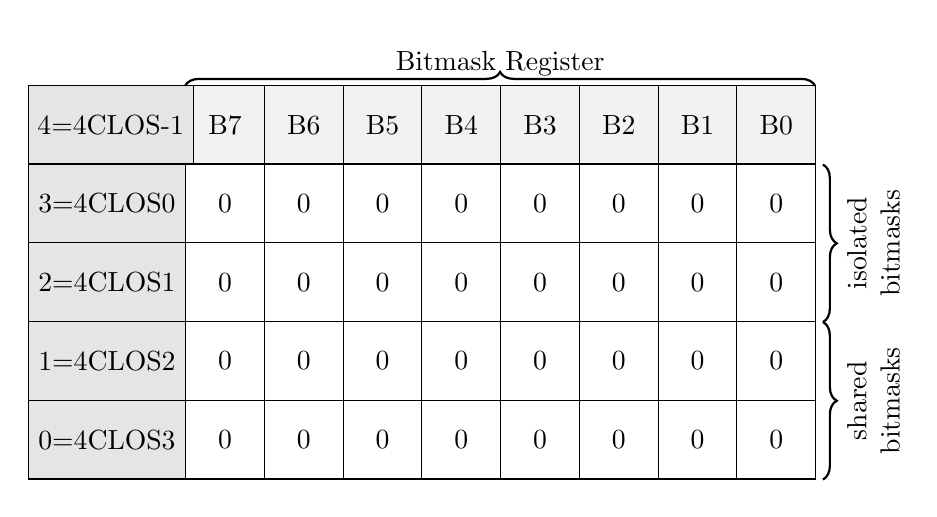
\begin{tikzpicture}

	\foreach \x [evaluate = \bindex using int(8-\x)] in {1,...,8}
		    	\node at (\x,4)[rectangle, draw=black, fill=black!5, minimum height = 1cm, minimum width = 1cm, anchor=south west] (r1\x) 
							{B\bindex};

	\foreach \x in {1,...,8}
				{\ifthenelse{\x>5}
						{\node at (\x,3)[rectangle, draw=black, fill=green!20, minimum height = 1cm, minimum width = 1cm, anchor=south west] (r2\x) {\textbf{1}};}
						{\node at (\x,3)[rectangle, draw=black, fill=white, minimum height = 1cm, minimum width = 1cm, anchor=south west] (r2\x) {0};}

				}
	
		    	%\node at (\x,3)[rectangle, draw=black, fill=white, minimum height = 1cm, minimum width = 1cm, anchor=south west] (r2\x) 
				%			{\ifthenelse{\x>5}{\textbf{1}}{0}};

	\foreach \x in {1,...,8}
				{\ifthenelse{\x>2 \AND \x<6}
						{\node at (\x,2)[rectangle, draw=black, fill=pink!30, minimum height = 1cm, minimum width = 1cm, anchor=south west] (r3\x) {\textbf{1}};}
						{\node at (\x,2)[rectangle, draw=black, fill=white, minimum height = 1cm, minimum width = 1cm, anchor=south west] (r3\x) {0};}
				}
	
		
		    	%% \node at (\x,2)[rectangle, draw=black, fill=white, minimum height = 1cm, minimum width = 1cm, anchor=south west] (r3\x) 
				%%			{\ifthenelse{\x>2 \AND \x<6}{\textbf{1}}{0}};

	\foreach \x in {1,...,8}
				{\ifthenelse{\x<3}
						{\node at (\x,1)[rectangle, draw=black, fill=Blue!10, minimum height = 1cm, minimum width = 1cm, anchor=south west] (r4\x) {\textbf{1}};}
						{\node at (\x,1)[rectangle, draw=black, fill=white, minimum height = 1cm, minimum width = 1cm, anchor=south west] (r4\x) {0};}

				}		    
				%% \node at (\x,1)[rectangle, draw=black, fill=white, minimum height = 1cm, minimum width = 1cm, anchor=south west] (r4\x) 
				%% 			{\ifthenelse{\x<3}{\textbf{1}}{0}};


	\foreach \x in {1,...,8}
				{\ifthenelse{\x<3}
						{\node at (\x,0)[rectangle, draw=black, fill=Blue!10, minimum height = 1cm, minimum width = 1cm, anchor=south west] (r5\x) {\textbf{1}};}
						{\node at (\x,0)[rectangle, draw=black, fill=white, minimum height = 1cm, minimum width = 1cm, anchor=south west] (r5\x) {0};}

				}	
		    	%% \node at (\x,0)[rectangle, draw=black, fill=white, minimum height = 1cm, minimum width = 1cm, anchor=south west] (r5\x) 
				%% 			{\ifthenelse{\x<3}{\textbf{1}}{0}};


	\foreach \y [evaluate = \closindex using int(3-\y)] in {4,...,0}
		    	\node at (-1,\y)[rectangle, draw=black, fill=black!10, minimum height = 1cm, minimum width = 2cm, anchor=south west] (r6\y) 
							{\ifthenelse{\y=4}{CLOS}{\closindex}};

	\draw[thick, decorate, decoration={brace,mirror,amplitude=5pt}] (9.1,2) -- (9.1,4) node [below, align=center, midway, rotate=90, text width=2cm] {\\isolated bitmasks};
	\draw[thick, decorate, decoration={brace,mirror,amplitude=5pt}] (9.1,0) -- (9.1,2) node [below, align=center, midway, rotate=90, text width=2cm] {\\shared bitmasks};

	\draw[thick, decorate, decoration={brace,amplitude=5pt}] (1,5) -- (9,5) node [above, align=center, midway] {\\Bitmask Register};

	%\node (isolatedmasks) at (11, 3) [text width=3cm, align=right]{Isolated Bitmasks};
	%\node (sharedmasks) at (11, 1) [text width=3cm, align=right]{Shared Bitmasks};	

	%\begin{scope}[>=latex]
	%\draw [thick, ->] (r28) to [bend left=45] (isolatedmasks.center);
	%\draw [thick, ->] (r38) to [bend left=45] (isolatedmasks.center);
	%\end{scope}

\end{tikzpicture}
\end{center}
\ifreport
\caption{Example of LLC Partitioning via Bitmasks. Three cache partitions are created by the bitmask registers. 
		First two are isolated ($3/8$ of LLC each) from the rest and the third is shared ($1/4$ of LLC).}
\fi
\label{fig-cat-bitmasks}
\end{figure}

Figure \ref{fig-cat-bitmasks} shows an example where capacity bitmask registers are shown for four applications. The first two masks are 
an example where LLC partitions are isolated. The last two masks give an example where LLC is shared by two applications.

The feature can be used to isolate a real-time guest cache from other guests to ensure any accesses to LLC from GPOS
will not pollute the cache of the real-time application. Figure \ref{fig-cat-isolated} gives an example scenario where virtualized software system
uses cache allocation feature to partition LLC of four guests according to bitmasks given in Figure \ref{fig-cat-bitmasks}.
\begin{figure}[!htb]
\begin{center}
\begin{tikzpicture}


%\draw[step=0.5cm, gray, very thin] (0,0) grid (9,9);


\node at (0,5.5) [rectangle, draw=black, thick, fill=black!3, rounded corners,  postaction={pattern= dots, pattern color=black!50}, minimum height = 2cm, minimum width = 1cm, anchor=south west] (g1) {g1};
\node at (1.25,5.5) [rectangle, draw=black, fill=black!3, thick, rounded corners, postaction={pattern=  dots, pattern color=black!50}, minimum height = 2cm, minimum width = 1cm, anchor=south west] (g2) {g2};
\node at (2.5,5.5) [rectangle, draw=black, fill=black!3, thick, rounded corners, postaction={pattern= dots, pattern color=black!50}, minimum height = 2cm, minimum width = 1cm, anchor=south west] (gN) {g3};
\node at (3.75,5.5) [rectangle, draw=black, fill=black!3, thick, rounded corners, postaction={pattern=  dots, pattern color=black!50}, minimum height = 2cm, minimum width = 1cm, anchor=south west] (gN) {g4};

\node at (6,5.5) [rectangle, draw=black, fill=black!3, thick, rounded corners, postaction={pattern= north east lines, pattern color=black!50}, minimum height = 2cm, minimum width = 1cm, anchor=south west] (g1) {g1};
\node at (7.25,5.5) [rectangle, draw=black, fill=black!3, thick, rounded corners, postaction={pattern= north west lines, pattern color=black!50}, minimum height = 2cm, minimum width = 1cm, anchor=south west] (g2) {g2};
\node at (8.5,5.5) [rectangle, draw=black, fill=black!3, thick, rounded corners, postaction={pattern= dots, pattern color=black!50}, minimum height = 2cm, minimum width = 1cm, anchor=south west] (gN) {g3};
\node at (9.75,5.5) [rectangle, draw=black, fill=black!3, thick, rounded corners, postaction={pattern= dots, pattern color=black!50}, minimum height = 2cm, minimum width = 1cm, anchor=south west] (gN) {g4};

\node at (0,4) [rectangle, draw=black, thick, rounded corners, fill=black!3, minimum height = 1cm, minimum width = 5cm, anchor=south west] (hypervisor1) {Hypervisor} ;
\node at (6,4) [rectangle, draw=black, thick, rounded corners, fill=black!3, minimum height = 1cm, minimum width = 5cm, anchor=south west] (hypervisor2) {Hypervisor} ;

\node at (0,2.5) [rectangle, draw=black, thick, rounded corners, fill=black!5, minimum height = 1cm, minimum width = 5cm, anchor=south west] (cores2) {Processor};
\node at (6,2.5) [rectangle, draw=black, thick, rounded corners, fill=black!5, minimum height = 1cm, minimum width = 5cm, anchor=south west] (cores2) {Processor};

\node at (0,0) [rectangle, draw=black, thick, fill=black!3, rounded corners, postaction={pattern= dots, pattern color=black!50}, minimum height = 2cm, minimum width = 5cm, anchor=south west] (llc1) {shared LLC (g1, g2, g3, g4)};
\node at (6,0) [rectangle, draw=black, thick, rounded corners, fill=black!3, minimum height = 2cm, minimum width = 5cm, anchor=south west] (llc2) {};

\node at (6,0) [rectangle, draw=black!20, very thin, rounded corners, postaction={pattern= north east lines, pattern color=black!50}, minimum height = 2cm, minimum width = 1.5cm, anchor=south west] (g1llc) {g1};
\node at (7.5,0) [rectangle, draw=black!20,  very thin, rounded corners,postaction={pattern= north west lines, pattern color=black!50}, minimum height = 2cm, minimum width = 1.5cm, anchor=south west] (g2llc) {g2};
\node at (9,0) [rectangle, draw=black!20,  very thin, rounded corners,  postaction={pattern= dots, pattern color=black!50}, minimum height = 2cm, minimum width = 2cm, anchor=south west] (g23llc) {g2, g3};

\draw [decorate, decoration={random steps,segment length=3pt,amplitude=1pt}] (5.5,-0.2) -- (5.5,7.7);

\end{tikzpicture}
\end{center}
\ifreport
\caption{Comparison of shared and isolated LLC. One the left is virtual setup when LLC is shared by four guests. On the right is a virtual setup that uses bitmasks from Figure \ref{fig-cat-bitmasks}}
\fi
\label{fig-cat-isolated}
\end{figure}



\section{PHIDIAS Hypervisor}
Provable Hypervisor with Integrated Development Information (PHIDIAS) is a multikernel based hypervisor specifically designed to host real-time applications \cite{nordholz2017design}. 
PHIDIAS hypervisor follows design principles that make it suitable for real-time systems. 
The hypervisor supports multi-core architectures ARM, x86, and MIPS. This section will provide a brief description of Phidias hypervisor design, 
implementation on x86 architecture and the mechanisms provided to guest OS.

\subsection{Multikernel Architecture}
Baumann et. al. introduced the idea of multikernel OS architecture for multicore and heterogeneous computer architectures \cite{baumann2009multikernel}. 
Their approach removes the requirement of synchronization primitives between software parts executing on different cores by removing the shared memory.
The design approach supports sharing of data between cores using explicit message passing communication primitives.
Phidias uses multikernel design approach where each physical core of the processor runs an instance of Phidias microkernel.
Every instance of the kernel runs in its own address space.
The code is shared by all instances but data is private to each instance.
There are some exceptions though, few variables are shared to implement locks for shared devices like UART.
The hypervisor kernel instance manages virtual machines and only this instance has access to the virtual machine state.
The multikernel model greatly simplifies the design of hypervisor and removes the need of synchronization primitives, 
hence reducing the complexity of the hypervisor.
The multikernel design approach is a matching solution for virtual machines as each VM is running in isolation from rest of the VMs.
In order to support communication between different virtual machines, Phidias supports 
asynchronous communication based on explicit message passing and shared memory buffers.

\subsection{Principle of Staticity}
The key design principle used to develop PHIDIAS is the principle of staticity.
Jan Nordholz in his Ph.D. thesis \cite{nordholz2017design} has defined the principle of staticity as follows:
\emph {"A hypervisor implementation for an embedded system can
and should be meticulously tailored to its usage scenario. Thus
every element of dynamicity that does not constitute a mandatory
part of runtime functionality is to be transformed into a
compile-time configuration tool. The retained runtime code is
then purely static, its actions determined by previously generated and externally verifiable configuration data."}

Every real-time embedded application has different requirements and requires a custom-tailored solution for the use case. 
Many real-time systems go through rigorous testing before they are deployed in the field and require the designers to prove their correctness.
The principle of staticity states that an embedded hypervisor should have no dynamic component, or minimal if there is no other way around.
Phidias uses the principle of staticity as a key design rule to ease software provability and reduce run time complexity. 
Removing the dynamic components from the hypervisor also reduces its footprint which is very attractive for embedded application with limited
memory resources.
The principle of staticity requires that all types of memory requests needed for the virtual machine and devices are known 
before integration of the software systems.

The Phidias hypervisor uses an XML based system configuration tool to create virtual machine configuration and generate the core of the hypervisor.
Phidias supports static partitioning of hardware resources. 
Each guest operating system is assigned a subset of processing elements, memory space, and IO devices.
Figure \ref{fig-static-part} shows an example configuration scenario where CPU cores and memory divided among the guests.
The principle of staticity is used by Phidias to completely remove memory allocation system.
The memory allocator is removed by creating static page-tables from system descriptions, for both the hypervisor and the virtual machines.
The device emulation core also uses principle of staticity to create and add custom tailored emulation core,
hence reducing the runtime complexity.

\begin{figure}[!htb]
\begin{center}
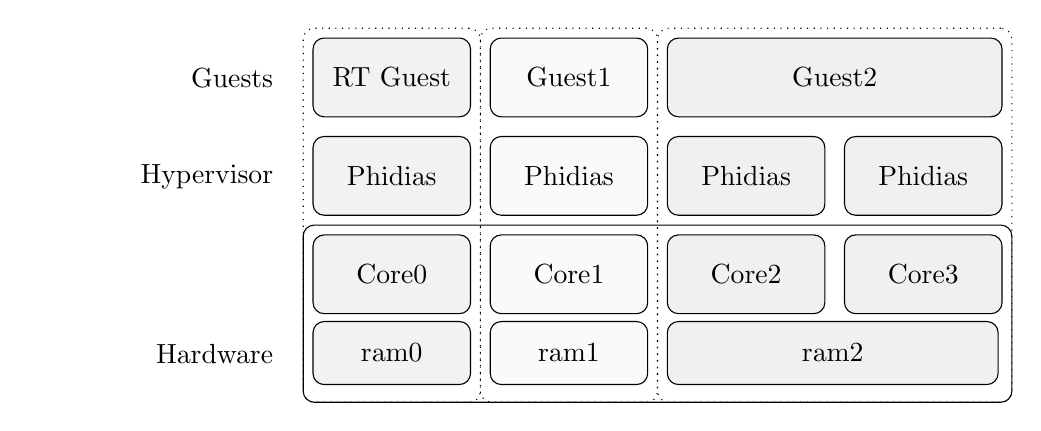
\begin{tikzpicture}

\node at (0,0)[rectangle, draw=black, fill=black!5, rounded corners, minimum height = 1cm, minimum width = 2cm, anchor=south west] (core0) {Core0};
\node at (2.25,0)[rectangle, draw=black, fill=black!2, rounded corners, minimum height = 1cm, minimum width = 2cm, anchor=south west] (core1) {Core1};
\node at (4.50,0)[rectangle, draw=black, fill=black!6, rounded corners, minimum height = 1cm, minimum width = 2cm, anchor=south west] (core2) {Core2};
\node at (6.75,0)[rectangle, draw=black, fill=black!6, rounded corners, minimum height = 1cm, minimum width = 2cm, anchor=south west] (core3) {Core3};

\node at (0,-0.9) [rectangle, draw=black, fill=black!5, rounded corners, minimum height = 0.8cm, minimum width = 2cm, anchor=south west] (ram0) {ram0};
\node at (2.25,-0.9) [rectangle, draw=black, fill=black!2, rounded corners, minimum height = 0.8cm, minimum width = 2cm, anchor=south west] (ram1) {ram1};
\node at (4.50,-0.9) [rectangle, draw=black, fill=black!6, rounded corners, minimum height = 0.8cm, minimum width = 4.2cm, anchor=south west] (ram2) {ram2};

\begin{scope}[fill opacity=0.0]
\node at (-0.125,-0.125-1)[rectangle, draw=black, fill=white, rounded corners, minimum height = 2.25cm, minimum width = 9.00cm, anchor=south west] (hardware) {};

\node at (-0.125,-1.125)[rectangle, draw=black, fill=black!5, dotted, rounded corners, minimum height = 4.75cm, minimum width = 2.25cm, anchor=south west] (rtg) {};
\node at (2.125,-1.125)[rectangle, draw=black, fill=black!2, dotted, rounded corners, minimum height = 4.75cm, minimum width = 2.25cm, anchor=south west] (g1) {};
\node at (4.375,-1.125)[rectangle, draw=black, fill=black!6, dotted, rounded corners, minimum height = 4.75cm, minimum width = 4.50cm, anchor=south west] (g2) {};

\end{scope}

\node at (0.0,1.25)[rectangle, draw=black, fill=black!5, rounded corners, minimum height = 1cm, minimum width = 2cm, anchor=south west] {Phidias};
\node at (2.25,1.25)[rectangle, draw=black, fill=black!2, rounded corners, minimum height = 1cm, minimum width = 2cm, anchor=south west] {Phidias};
\node at (4.50,1.25)[rectangle, draw=black, fill=black!6, rounded corners, minimum height = 1cm, minimum width = 2cm, anchor=south west] {Phidias};
\node at (6.75,1.25)[rectangle, draw=black, fill=black!6, rounded corners, minimum height = 1cm, minimum width = 2cm, anchor=south west] {Phidias};

\node at (0.0,2.5)[rectangle, draw=black, fill=black!5, rounded corners, minimum height = 1cm, minimum width = 2cm, anchor=south west] {RT Guest};
\node at (2.25,2.5)[rectangle, draw=black, fill=black!2, rounded corners, minimum height = 1cm, minimum width = 2cm, anchor=south west] {Guest1};
\node at (4.50,2.5)[rectangle, draw=black, fill=black!6, rounded corners, minimum height = 1cm, minimum width = 4.25cm, anchor=south west] {Guest2};

\node (hardware) at (-2.0, -0.5) [text width=3cm, align=right]{Hardware};
\node (phidias) at (-2.0, 1.75) [text width=3cm, align=right]{Hypervisor};
\node (guests) at (-2.0, 3.0) [text width=3cm, align=right]{Guests};

\end{tikzpicture}
\end{center}
\ifreport
\caption{Example partitioning of a multicore x86 platform using Phidias. The guest are allocated separate CPU cores and RAM memory. 
Since Phidias follows multikernel design approach, a clone of Phidias runs on each core.}
\fi
\label{fig-static-part}
\end{figure}


\subsection{Non-Preemptible Kernel}
Phidias hypervisor kernel is non-preemptible and interrupts are always disabled when hypervisor executes. 
Preemptibility means a higher priority task can preempt currently running task until it finishes and lower priority task is then resumed.
An RTOS is always designed to be preemptible, even the GPOS also provide voluntary preemption.

Preemptible kernels sound great, however, it is achieved at the cost of higher software complexity.  
It introduces new execution paths in the kernel and makes it difficult to prove the correctness of the software system.
Since the software can be preempted at any point by a high priority task the kernel has to support context switching and
synchronization primitives to ensure correct software behavior.

Non-preemptibility can be tolerated if all execution paths in the hypervisor are kept short.
Phidias has the capability to keep its execution paths short.
The only synchronization primitive used by the Phidias is to multiplex UART device which is shared among the guests. 
Since UART is an important device that helps to print debug information the synchronization locks were required for multiplexing UART.
However, it is highly unlikely that the guests would compete for UART except during the bootup time.
Phidias also support partitioning of hardware resources, that helps to keep the emulation paths short.
Furthermore, the availability of multiple cores allows Phidias to partition CPU resources on the core basis. 
In order to guarantee deterministic response times for real-time guests, Phidias can dedicate hardware resources to the real-time guest.
Assigning dedicated cores to real-time guests allows Phidias to completely remove scheduling overhead and overhead of APIC emulation software.

To keep low software complexity and footprint preemption is not supported by Phidias.
Phidias hypervisor kernel paths are very short that simplifies the software design and makes it easier to prove correctness.

\subsection{Inter-VM Communication}
Phidias supports asynchronous communication between virtual machines.
Virtual machines can transfer data between each other through communication channels that
are configured statically before deploying software system.
A communication channel consists of shared buffer and a virtual interrupt for signaling.
The VM stores data in a shared buffer and generates an interrupt to inform receiver.
Phidias injects a virtual interrupt to the receiving VM to inform availability of data.
Phidias does not support creation of communication channels at the runtime.

\subsection{Small TCB}
Since Phidias uses principle of staticity that eliminates dynamic parts and non-preemptive
kernel to reduce hypervisor complexity, the resulting hypervisor has very small code size.
The small code size of the hypervisor results in small trusted computing base (TCB).
Small TCB increases the confidence in software system's security.
Since the number of bugs in a software is proportional to code lines in the software\cite{lipow1982number}, 
a small TCB reduces the potential security risks.
It also makes it easier to test and maintain the hypervisor.


\subsection{Guest Device Handling} 
Phidias hypervisor supports three mechanisms to interface guest devices, a brief introduction to each mechanism is provided in this section.
Figure \ref{fig-device-handling} shows the difference between the three device handling mechanisms supported.
\begin{figure}[!htb]
\begin{center}
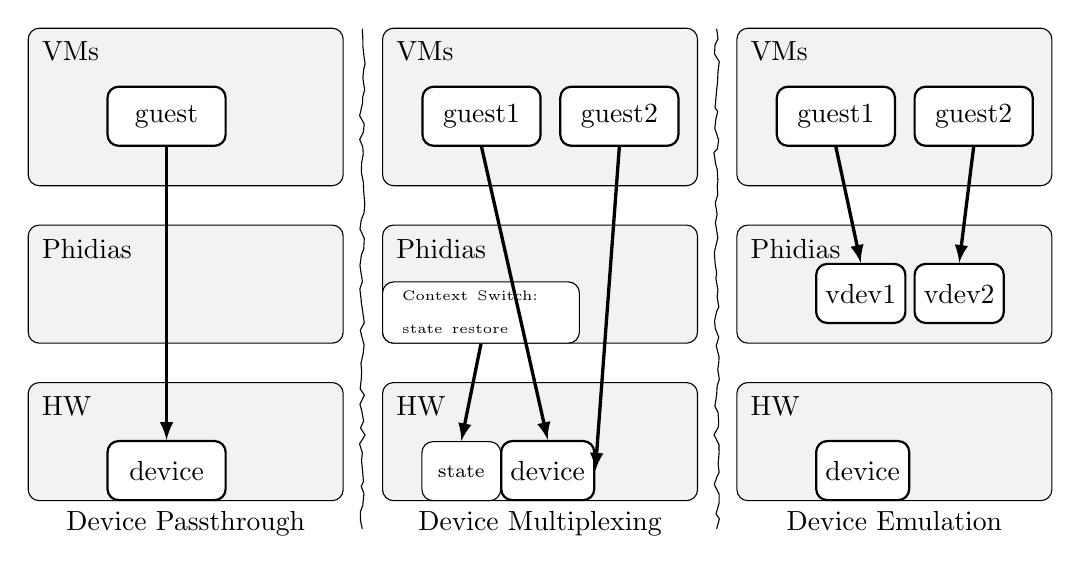
\begin{tikzpicture}

\node at (0,4)[rectangle, draw=black, fill=black!5, rounded corners, minimum height = 2cm, minimum width = 4cm, anchor=south west] (vms1) {};
\node[below right, inner sep=5pt] at (vms1.north west) {VMs};
\node at (4.5,4)[rectangle, draw=black, fill=black!5, rounded corners, minimum height = 2cm, minimum width = 4cm, anchor=south west] (vms2) {};
\node[below right, inner sep=5pt] at (vms2.north west) {VMs};
\node at (9,4)[rectangle, draw=black, fill=black!5, rounded corners, minimum height = 2cm, minimum width = 4cm, anchor=south west] (vms3) {};
\node[below right, inner sep=5pt] at (vms3.north west) {VMs};

\node at (0,2)[rectangle, draw=black, fill=black!5, rounded corners, minimum height = 1.5cm, minimum width = 4cm, anchor=south west] (phidias1) {};
\node[below right, inner sep=5pt] at (phidias1.north west) {Phidias};
\node at (4.5,2)[rectangle, draw=black, fill=black!5,  rounded corners, minimum height = 1.5cm, minimum width = 4cm, anchor=south west] (phidias2) {};
\node[below right, inner sep=5pt] at (phidias2.north west) {Phidias};
\node at (9,2)[rectangle, draw=black, fill=black!5, rounded corners, minimum height = 1.5cm, minimum width = 4cm, anchor=south west] (phidias3) {};
\node[below right, inner sep=5pt] at (phidias3.north west) {Phidias};

\node at (0,0)[rectangle, draw=black, fill=black!5, rounded corners, minimum height = 1.5cm, minimum width = 4cm, label=south:Device Passthrough,anchor=south west] (hw1) {};
\node[below right, inner sep=5pt] at (hw1.north west) {HW};
\node at (4.5,0)[rectangle, draw=black, fill=black!5, rounded corners, minimum height = 1.5cm, minimum width = 4cm, label=south:Device Multiplexing, anchor=south west] (hw2) {};
\node[below right, inner sep=5pt] at (hw2.north west) {HW};
\node at (9,0)[rectangle, draw=black, fill=black!5, rounded corners, minimum height = 1.5cm, minimum width = 4cm, label=south:Device Emulation, anchor=south west] (hw3) {};
\node[below right, inner sep=5pt] at (hw3.north west) {HW};

\node at (1,4.5)[thick, rectangle, draw=black, fill=white, rounded corners, minimum height = 0.75cm, minimum width = 1.5cm, anchor=south west] (g11) {guest};
\node at (1,0)[thick, rectangle, draw=black, fill=white, rounded corners, minimum height = 0.75cm, minimum width = 1.5cm, anchor=south west] (dev1) {device};
\begin{scope}[>=latex]
	\draw [very thick, ->] (g11.south) to [bend right=0] (dev1.north);
\end{scope}

\node at (5,4.5)[thick, rectangle, draw=black, fill=white, rounded corners, minimum height = 0.75cm, minimum width = 1.5cm, anchor=south west] (g21) {guest1};
\node at (6.75,4.5)[thick, rectangle, draw=black, fill=white, rounded corners, minimum height = 0.75cm, minimum width = 1.5cm, anchor=south west] (g22) {guest2};
\node at (4.5,2.0)[rectangle, draw=black, fill=white,  rounded corners, minimum height = 0.75cm, minimum width = 2.5cm, text width=2cm, anchor=south west] (hyp2st) 
					{\tiny{Context Switch: state restore}};
\node at (5,0)[rectangle, draw=black, fill=white, rounded corners, minimum height = 0.75cm, minimum width = 1cm, anchor=south west] (dev2st) {\scriptsize{state}};
\node at (6,0)[thick, rectangle, draw=black, fill=white, rounded corners, minimum height = 0.75cm, minimum width = 1cm, anchor=south west] (dev2) {device};
\begin{scope}[>=latex]
	\draw [very thick, ->] (g21.south) to [bend right=0] (dev2.north);
	\draw [very thick, ->] (g22.south) to [bend right=0] (dev2.east);
	\draw [very thick, ->] (hyp2st.south) to [bend right=0] (dev2st.north);
\end{scope}


\node at (9.5,4.5)[thick, rectangle, draw=black, fill=white, rounded corners, minimum height = 0.75cm, minimum width = 1.5cm, anchor=south west] (g31) {guest1};
\node at (11.25,4.5)[thick, rectangle, draw=black, fill=white, rounded corners, minimum height = 0.75cm, minimum width = 1.5cm, anchor=south west] (g32) {guest2};
\node at (10,2.25)[thick, rectangle, draw=black, fill=white, rounded corners, minimum height = 0.75cm, minimum width = 1cm, anchor=south west] (vdev1) {vdev1};
\node at (11.25,2.25)[thick, rectangle, draw=black, fill=white, rounded corners, minimum height = 0.75cm, minimum width = 1cm, anchor=south west] (vdev2) {vdev2};
\node at (10,0)[thick, rectangle, draw=black, fill=white, rounded corners, minimum height = 0.75cm, minimum width = 1cm, anchor=south west] (dev3) {device};
\begin{scope}[>=latex]
	\draw [very thick, ->] (g31.south) to [bend right=0] (vdev1.north);
	\draw [very thick, ->] (g32.south) to [bend right=0] (vdev2.north);	
\end{scope}

\draw [decorate, decoration={random steps, segment length=3pt,amplitude=1pt}] (4.25,-0.35) -- (4.25,6);
\draw [decorate, decoration={random steps, segment length=3pt,amplitude=1pt}] (8.75,-0.35) -- (8.75,6);

\end{tikzpicture}
\end{center}
\ifreport
\caption{Device handling mechanisms supported by Phidias}
\fi
\label{fig-device-handling}
\end{figure}


\subsubsection{Device Passthrough}
The device passthrough mechanism allows a guest to take complete ownership of a device. 
The virtual machine interacts with the device without any intervention from the hypervisor.
Memory mapped devices are passed to the guest by giving complete ownership of the device memory region. 
In this case, the Phidias configuration tool enables addition of an entry in statically allocated nested page-tables of the owner guest 
for exclusive read/write accesses of the device memory.
On contrary, some devices are IO mapped, in which case exclusive access to that IO region is given to the owner guest.
The device passthrough mechanism results in highest performance however it is suitable only when a guest exclusively owns the device.

\subsubsection{Device Multiplexing}
If the same device is accessed from multiple guests then Phidias hypervisor supports multiplexing of the device between guests. 
Device multiplexing is achieved by restoring the device state for a guest whenever context switch takes place. 
The current state of the device is saved until the context switch happens again. 
Saving and restoring device state on context switch add small overhead however once completed the device can be accessed exclusively by the guest OS.
This mechanism can only be supported for devices that are virtualization aware and expose their complete state.
Another situation when this mechanism becomes useful is when the guests use the same state for the device, in such scenario even the overhead of 
state restore can be saved. 
An example is UART used by the guests for command-line input/output.
Typical interaction of guest with UART includes one-time configuration at boot-up and
and later use it to dump debugging information.
Phidias supports multiplexing of UART device. The UART is configured once at boot-up by the Phidias and guests
are informed using kernel command-line argument to use preconfigured baudrate. 
All accesses to UART device from guests are multiplexed by Phidias.

\subsubsection{Device Emulation}
Device emulation is the only choice of device handling if the device does not exist on the hardware or it is not virtualization-aware.
The behavior of the device is completely emulated by the hypervisor in software and guest OS is oblivious to the fact that device does not exist on the hardware.
All requests to the target device are trapped and emulated by the host software. This mechanism has the largest overhead due to emulation of the device in software.

\subsubsection{Static Configuration Tool}
Phidias hypervisor kernel itself is created through a static configuration tool. 
As stated earlier, the hypervisor uses the principle of staticity as the main design goal to ease provability and lower the software complexity.
The principle of staticity requires all configuration of the hypervisor kernel and virtual machines to be enlisted prior to the creation of hypervisor executable. 
The static configuration tool takes the configuration as input and creates all necessary data structures to configure the hypervisor microkernel. 
The configuration tool also generates page-tables data structures for the hypervisor and nested page-tables for each virtual machine. 
All page-table structures are transformed to binary and packaged into the final executable of the software system.


\subsection{Implementation on x86}
This section will give a brief overview of Phidias implementation on Intel x86 platform.

Phidias utilizes Intel virtualization extensions to implement faithful virtualization. 
It uses extended page-table (Intel EPT) feature for MMU virtualization. 
And supports per core local APIC virtualization through software
emulation or by using hardware virtualization technique for APIC virtualization (APIC-v).

The hypervisor executes in VM root operation mode and launches virtual machines that run in VM non-root operation mode.
Hypervisor configures virtual machine control structure (VMCS) to cause vmexit transition if the guest tries to execute an IO operation, on arrival of an external interrupt, and or guest tries to execute of a privileged instruction.  
The hypervisor takes control when such a situation occurs, emulates the desired behavior and returns control back to the virtual machine through the vmentry transition. 
Phidias only handles exceptions for nested page-tables, the guest has complete control over exceptions that may occur on guest page-tables.
The nested page-table exceptions are configured as traps and used to emulate device accesses. 

Recent Intel virtualization extensions support optimizing hypervisor operation for guest access to machine specific registers and IO ports through bitmaps.
Phidias hypervisor supports all these mechanisms to lower virtualization overhead. 

In order to perform useful operations, a Linux guest requires a least four devices: a timer as clock-source, a timer for event generation, an interrupt controller, and a serial interface for input/output. The event generation and clock source timers can use the same timer infrastructure, however, on x86 these two can be different. Phidias supports these minimal set of devices per guest, details of implementation follows:

\subsubsection{Interrupt Controller}
An interrupt controller is a programmable logic circuit inside the microprocessor chip that allows processor core to configure and control interrupts.
CPU associates an individual interrupt source with an interrupt vector by writing the vector number into the corresponding interrupt controller register.
This interrupt vector number is given to the processor by interrupt controller when an interrupt arrives from the particular source, which allows CPU to
recognize the source of interrupt. The interrupt controller also allows CPU to disable an individual interrupt.

The x86 multiprocessor architecture supports two types of interrupt controllers.
An interrupt controller per physical CPU core, known as local advanced programmable interrupt controller (LAPIC).
And at least one interrupt controller to configure interrupts from external IO devices, known as IOAPIC.
LAPIC is used to configure interrupts local to CPU core and to send and receive inter-processor interrupts (IPIs).
IOAPIC is used to receive interrupts from devices external to the multiprocessor chip.
Some external devices also send interrupts to the microprocessor chip on the system bus, these interrupt are called Message Signaled Interrupts (MSIs).
Interrupts delivered by PCIe cards is an example of this type of interrupt.
LAPIC is responsible to decode these interrupts and forward them to the core.

Phidias hypervisor supports emulation of local APIC in software. 
In this case, a software state of APIC is maintained for the guest while the actual hardware is in full control of the hypervisor.
Phidias also supports hardware-based APIC virtualization (APIC-v).
The APIC virtualization feature allows reducing software emulation time by emulating read/write access in hardware.
The processor keeps track of virtual APIC core and allows virtual interrupt delivery without hypervisor intervention.

The IOAPIC interrupt controller is emulated by Phidias in software by keeping a software state of IOAPIC. 
External interrupts are received by Phidias and virtual IOAPIC states of each guest are consulted to inject and a virtual interrupt to that guest.
The hypervisor supports two types of virtual interrupt injection mechanisms.
When an interrupt source is shared between guests, the hypervisor injects virtual interrupts to the guests.
If a guest is the only owner of the interrupt, it allows interrupt passthrough or direct interrupt injection using APIC virtualization.
When interrupt passthrough is used then hypervisor takes the interrupt and passes it to the hypervisor without further processing, keeping the kernel execution path short. 
When direct interrupt injection is used, the hypervisor uses APIC virtualization to inject virtual interrupt to the guest without hypervisor intervention.

\subsubsection{Timer as Event Generator}
Linux guest on x86 platform uses per core local APIC timer (LAPIC timer) to generate events. 
The local APIC core supports various modes of operation for event generation: periodic, one-shot or TSC-deadline mode. 
Phidias uses LAPIC timer core to emulate guest timer events.
It has a generic timer infrastructure to generate timer events and supports all modes of operations desired by the guest. 
The timer infrastructure keeps a queue of time events sorted by the event deadline.
Event with the earliest deadline is programmed into the LAPIC timer, when the timer expires the event is forwarded to the requesting guest.
The same timer event generation infrastructure is used by the hypervisor scheduler to trigger scheduling events.

\subsubsection{Timer as Clock Source}
In addition to event generation, Linux guest uses a monotonically increasing timer source as its clock-source. 
Guest uses this timer to keep track of time. 
On x86 platform Linux guest uses time-stamp counter (TSC) as the clock source. 
TSC increments monotonically at the processor clock speed and keeps the count value in a 64-bit register.
Phidias hypervisor support TSC counter as a pass-through device.
The current value of the TSC counter is always available to the guest without hypervisor intervention.
In order to keep the illusion that guest is running directly on the hardware, Phidias supports TSC-offsetting feature.
TSC-offsetting feature allows the host to offset the counter value to compensate for time quantum for which host executes on the hardware.
PHIDIAS configures the offset value to the time that lapses between vmexit and vmentry.

\subsubsection{Serial Interface}
A serial interface is very useful for a guest to interact with the user and dump debugging information.
Phidias hypervisor supports one serial interface per guest by emulating UART 16650 interface of the x86 architecture.
The hypervisor uses the same interface to dump its own debug information. 
The emulation works in conjunction with a small tool on the host side that supports multiplexing of the interface between the guests and the hypervisor itself.
The multiplexer tool opens up one console per guest and one for the hypervisor. When a request to dump information from a guest arrives the hypervisor
sends this debug information to the serial interface. A special code sequence is sent to the console every time the interface is switched between the guests.
The code sequence is used by the host tool to differentiate where to dump incoming information. 
Similarly, when the user wants to interact with a virtual machine, a special code sequence is sent to the hypervisor.
This time the code sequence helps hypervisor to decide to which guest the input shall be routed. 
